
\chapter{Learning from Wizard-of-Oz data}
\label{chap:wozlearning}

The previous chapter presented the formalism of probabilistic rules and described their practical instantiation as latent nodes of a graphical model. Probabilistic rules are generally associated to a number of parameters, which may either express probabilities over effects (for probability rules) or utilities associated with particular decisions (for utility rules). But where exactly do these probabilities and utilities come from?
\index{supervised learning}

This thesis develops two distinct approaches to this question. The present chapter concentrates on the first approach, which is grounded in supervised learning techniques. We demonstrate how rule parameters can be optimised to best imitate the action choices of a human expert through statistical estimation based on Wizard-of-Oz data. The next chapter will then detail an alternative reinforcement learning approach to the same task.

The chapter is divided in three sections.  Section \ref{sec:rule-params} describes how uncertainty regarding the value of rule parameters can be explicitly represented through prior distributions. Section \ref{sec:rule-supervised} goes on to explain how these distributions can be gradually refined on the basis of interaction data gathered from Wizard-of-Oz experiments.  Bayesian learning  is used to progressively narrow down the spread of the parameter distributions to the values providing the best fit for the observed data. Finally, Section \ref{sec:wozlearning-experiments} reports on experimental results in a human--robot interaction domain for which small amounts of Wizard-of-Oz data were recorded. The experiment compared the learning performance of a utility model structured with probabilistic rules against two baselines respectively encoded with plain utility tables and with linear models. The evaluation showed that the rule-structured model was able to imitate the dialogue policy followed by the wizard significantly better than its unstructured counterparts.

\section{Parameters of probabilistic rules}
\label{sec:rule-params}

\subsection{General methodology}

The examples of probabilistic rules seen so far all relied on fixed probability and utility values. These values can, however, be replaced by parameters that reflect unknown values that are to be estimated empirically, on the basis of training data. 
 
The overall structure of parametrised rules remains essentially identical to the one outlined in the previous chapter.  Probability rules are once more defined in terms of conditions $c_i$ associated to probability distributions $P(E_i)$ over effects.  The probability of each effect $e_{(i,j)}$ is, however, no longer fixed but is instead represented by a parameter $\theta_{(i,j)}$, giving rise to the following skeleton: 
\begin{equation}
\begin{aligned}
& \textbf{if} \ \ (c_{1}) \ \ \textbf{then} \\ 
& \;\;\;\;\; \begin{cases}
P(E_1\!=\!e_{(1,1)}) = \theta_{(1,1)} \\
 \dots \\
P(E_1\!=\!e_{(1,m_1)}) = \theta_{(1,m_1)} 
\end{cases} \\[3mm]
%& \textbf{else if} \ \ (c_{2}) \ \ \textbf{then} \\ 
%& \;\;\;\;\; \begin{cases}
%P(E_2\!=\!e_{(2,1)}) = \theta_{(2,1)}, \\
% \dots \\
%P(E_2\!=\!e_{(2,m_2)}) = \theta_{(2,m_2)}
%\end{cases} \\ 
& \dots  \\
& \textbf{else} \\
& \;\;\;\;\; \begin{cases}
P(E_{n}\!=\!e_{(n,1)}) = \theta_{(n,1)} \\
\dots \\
P(E_{n}\!=\!e_{(n,m_n)}) = \theta_{(n,m_n)}
\end{cases}
\end{aligned}
\end{equation}

Analogously, parametrised utility rules replace utility values with unknown parameters:
\begin{equation}
\begin{aligned}
& \textbf{if} \ \ (c_{1}) \ \ \textbf{then} \\ 
& \;\;\;\;\; \begin{cases}
U_1(d_{(1,1)}) = \theta_{(1,1)} \\
 \dots \\
U_1(d_{(1,m_1)}) = \theta_{(1,m_1)}
\end{cases} \\[3mm]
%& \textbf{else if} \ \ (c_{2}) \ \ \textbf{then} \\ 
%& \;\;\;\;\; \begin{cases}
%U_2(d_{(2,1)}) = \theta_{(2,1)} \\
% \dots \\
%U_2(d_{(2,m_2)}) = \theta_{(2,m_2)}
%\end{cases} \\
& \dots  \\
& \textbf{else} \\
& \;\;\;\;\; \begin{cases}
U_n(d_{(n,1)}) = \theta_{(n,1)} \\
\dots \\
U_n(d_{(n,m_n)}) = \theta_{(n,m_n)}
\end{cases}
\end{aligned}
\end{equation} 

We focus in this work on the problem of parameter estimation given a known and fixed rule structure.  The methodological standpoint adopted in this thesis rests on the idea that the structure of probabilistic rules is best determined by the system designer, while the rule parameters are best derived by statistical optimisation techniques. Based on our own practical experience with various dialogue systems, we believe that such a division of labour between the human designer and the learning algorithm is a sensible one, as system designers generally have a good grasp of the domain structure and relations between variables but are often unable to quantify the precise probability of an effect or utility of an action.\footnote{Humans are indeed notoriously poor at estimating probabilities and are prone to multiple cognitive biases when doing so, as evidenced by numerous studies in behavioural psychology.  \cite{ohagan2006} provides more details on the human perception of uncertainty and the difficult problem of probability elicitation from experts.}\index{probability distribution!elicitation of}

Although our work concentrates on parameter estimation \index{parameter estimation} with a known rule structure, it should be noted that recent developments in statistical relational learning have shown that the structure of stochastic rules can also be extracted from data \citep{PasulaZK07,Kok:2009}.\index{statistical relational learning}  These methods are, however, generally confined to domains of limited size and full observability and are therefore difficult to apply to the dialogue domains investigated in this thesis work.  

%Domain models can be composed of both fixed and parametrised rules and can therefore accommodate a wide spectrum of learning tasks from fully statistical models with virtually no prior knowledge to manually designed models with only a handful of parameters. 

\subsection{Parameter priors}
\label{sec:rule-params-priors}
\index{rule parameters!Bayesian learning of}
\index{rule parameters!prior distributions of}

Throughout this thesis, we follow a \textit{Bayesian} approach to parameter estimation and associate the rule parameters with explicit prior distributions over their range of possible values.  These prior parameter distributions have a continuous range of values and can be either univariate or multivariate.  The benefits of Bayesian approaches compared to maximum likelihood methods are multiple:
\begin{enumerate} 
\item Bayesian methods allow domain knowledge to be directly included into the learning cycle through the use of informative priors (cf. discussion below). The system designers are thus able to bias the initial prior distributions according to their domain expertise.
\item Bayesian methods explicitly capture the model uncertainty both at the beginning and at the end of the learning process. The outputs of a Bayesian learning cycle are indeed full posterior distributions over the possible parameter values instead of being reduced to point estimates (as for maximum likelihood estimation).  The dialogue agent can therefore explicitly account for parameter uncertainty at runtime and use it to simultaneously learn, reason and act in its environment \citep{Ross:2011}. Furthermore, the reliance on full parameter distributions facilitates the combination of multiple learning processes, as the posterior distribution generated by one learner can be passed on as the prior distribution of another. 
\end{enumerate}

We describe below possible parameter distributions for probability rules and then discuss the case of utility rules.  

\subsubsection*{Probability parameters}
\index{rule parameters!of probability rules}

The distributions over the effects of probability rules are categorical probability distributions.  As already discussed in Section \ref{sec:learning}, the parameter priors of categorical and multinomial distributions are best expressed using \textit{Dirichlet} distributions. \index{Dirichlet distribution}

Each distribution over effects $P(E_i)$ is associated with its own Dirichlet distribution of dimension $m_i$, where $m_i$ is the number of alternative effects (including the empty effect if appropriate).  Rule $r_{1}$ provides an example of a parametrised probability rule: 
\begin{align*}
r_{1}: \ \ \ \ \ & \textbf{if} \ (\mathit{Rain}\!=\!\mathit{false} \land \mathit{Weather}\!=\!\mathit{hot}) \ \textbf{then} \\
& \;\;\;\;\;  \begin{cases}
 P(\mathit{Fire}'\!=\!\mathit{true}) = \theta_{r_{1}(1,1)} \\ 
P(\mathit{Fire}'\!=\!\mathit{false}) = \theta_{r_{1}(1,2)}
\end{cases}  \\ 
& \textbf{else} \\
& \;\;\;\;\; \begin{cases}
P(\mathit{Fire}'\!=\!\mathit{true}) = \theta_{r_{1}(2,1)} \\
P(\mathit{Fire}'\!=\!\mathit{false}) = \theta_{r_{1}(2,2)}
\end{cases} 
\end{align*}


The parameters of rule $r_{1}$ can be expressed with two Dirichlets $\boldsymbol\theta_{r_{1}(1)} = \langle \theta_{r_{1}(1,1)},\theta_{r_{1}(1,2)} \rangle$ and $\boldsymbol\theta_{r_{1}(2)} = \langle \theta_{r_{1}(2,1)}, \theta_{r_{1}(2,2)} \rangle$ respectively associated with the effect distributions for the first and second condition.  The Dirichlet distributions in this example have two dimensions (since two alternative effects are mentioned in the rule), which make them equivalent to \textit{Beta} distributions. 

Dirichlet distributions are continuous, multivariate probability distributions defined by the meta-parameters $\boldsymbol\alpha = [\alpha_1, \dots, \alpha_k]$, where $k$ corresponds to the dimensionality of the categorical distribution of interest.  Dirichlet distributions over the parameters $\theta_1, \dots, \theta_k$ are formally expressed by the following probability density function:
\begin{align}
P(\theta_1, \dots, \theta_k\,; \boldsymbol\alpha) = \frac{1}{\mathrm{B}(\boldsymbol\alpha)} \prod_{i=1}^k \theta_i^{\alpha_i - 1} \ \ \ \text{with } \mathrm{B}(\boldsymbol\alpha) = \frac{\prod_{i=1}^k \Gamma(\alpha_i)}{\Gamma\bigl(\sum_{i=1}^k \alpha_i\bigr)}
\end{align}

where $ \mathrm{B}(\boldsymbol\alpha)$ serves as normalisation factor and builds upon the gamma function $\Gamma$.\footnote{The gamma function is a generalisation of the factorial for real numbers, and is defined as $\Gamma(z) = \int_0^\infty  t^{z-1} e^{-t}\,{\rm d}t$.} The notation $P(\theta_1, \dots, \theta_k\,; \boldsymbol\alpha)$ refers to the joint density function of the random variables $\theta_1, \dots, \theta_k$ given the specified (hyper-)parameters $\boldsymbol\alpha$. 

Figure \ref{fig:dirichletfun} depicts the shape of the probability density functions for several variants of the two-dimensional Dirichlet distribution $P(\theta_1,\theta_2\,; \boldsymbol\alpha)$ (also known as a Beta distribution).  The second dimension $\theta_2$ is not explicitly shown in the figure but can be directly derived from the first dimension, since $\theta_1 + \theta_2=1$.  The figure illustrates how the $\boldsymbol\alpha$ hyper-parameters determine the shape of the distribution. As the $\boldsymbol\alpha$ counts grow larger, the density function becomes increasingly focused on a particular region of the parameter space.  The $\boldsymbol\alpha$ counts can therefore be tuned to skew the distribution in a particular direction based on prior domain knowledge. Such prior distributions are called ``informative'' priors, since their shape is influenced by expert information. In the absence of such information, non-informative distributions such as $\mathrm{Dirichlet}(1,1)$ can also be employed. 
\index{informative and non-informative prior}
\begin{figure}[ht]
\centering
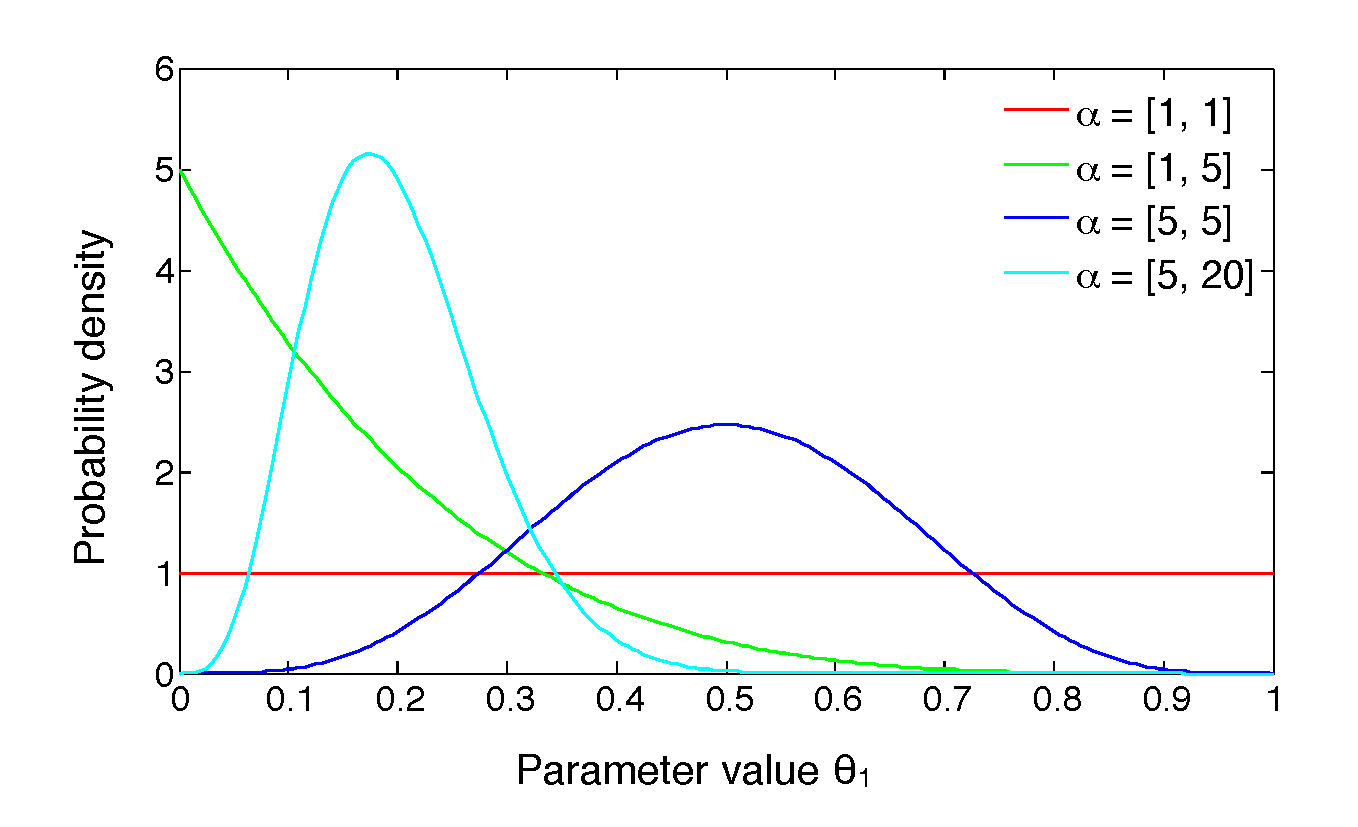
\includegraphics[scale=0.45]{imgs/dirichletfun.pdf}
\caption{Probability density functions for the Dirichlet distribution $P(\theta_1 \,; \boldsymbol\alpha)$  according to various values for the $\boldsymbol\alpha$ hyper-parameters.}
\label{fig:dirichletfun}
\end{figure}

As Dirichlet distributions are conjugate priors of categorical distributions, their posterior distribution after the observation of their corresponding variable remains a Dirichlet distribution with updated counts. As an illustrative example, the posterior distribution of $\boldsymbol\theta_{r_{1}(1)}$ after observing a fire when $\mathit{Rain}\!=\!\mathit{false} \land \mathit{Weather}\!=\!\mathit{hot}$ can be derived from Bayes' rule: 
\begin{align}
&P(\boldsymbol\theta_{r_{1}(1)} \; | \; \mathit{Fire}'\!=\!\mathit{true}, \mathit{Rain}\!=\!\mathit{false}, \mathit{Weather}\!=\!\mathit{hot}) \nonumber \\
& = \eta \ P(\mathit{Fire}'\!=\!\mathit{true} \; | \; \mathit{Rain}\!=\!\mathit{false}, \mathit{Weather}\!=\!\mathit{hot}\,; \boldsymbol\theta_{r_{1}(1)}) \ P(\boldsymbol\theta_{r_{1}(1)}) \nonumber \\
& = \eta \ \theta_{r_{1}(1,1)} \ \mathrm{Dirichlet}(\alpha_1,\alpha_2) \nonumber \\
& = \eta' \ \theta_{r_{1}(1,1)} \ [ \theta_{r_{1}(1,1)}^{\alpha_1 - 1} \times \theta_{r_{1}(1,2)}^{\alpha_2 - 1} ]   = \eta' \ \textrm{Dirichlet}(\alpha_1+1,\alpha_2) \nonumber 
\end{align}

where $\eta$ and $\eta'$ are normalisation factors.  Given a prior probability distribution $P(\boldsymbol\theta_{r_{1}(1)}) \sim \mathrm{Dirichlet}(\alpha_1, \alpha_2)$, the posterior distribution for $\boldsymbol\theta_{r_{1}(1)}$ after the observation  $\mathit{Fire}'\!=\!\mathit{true}$ is thus another Dirichlet distribution $\sim \mathrm{Dirichlet}(\alpha_1+1,\alpha_2)$.  This updated Dirichlet distribution results in a slightly higher probability for the occurrence of fire, reflecting the evidence provided by the observation. 

%As explained in Section \ref{sec:learning}, this property is, however, contingent on the full observability of the domain variables. 

%$For instance, we can encode the fact that the user is unlikely to change his intention after a clarification request by assigning a higher $\alpha$ value to the intention $i_u'$ corresponding to the current value $i_u$ when $a_m$ is a clarification request. 


\subsubsection*{Utility parameters}
\index{rule parameters!of utility rules}

The parameters of utility rules are also defined by probability density functions.  However, contrary to probability values, utility values are independent of one another and need not satisfy the probability axioms -- in particular, their possible values are not constrained to the range $[0,1]$ and the distribution does not need to sum up to $1$. Each utility value $u_{(i,j)}$ assigned to decision $d_{(i,j)}$ is therefore associated with its own, univariate distribution.

Rule $r_{2}$ illustrates a utility rule with four independent parameters:
\begin{align*}
r_{2}: \ \ & \textbf{if} \ (\mathit{Fire}\!=\!\mathit{true}) \ \textbf{then} \\
& \;\;\;\;\;  \begin{cases}
U(\mathit{Tanker}'\!=\!\mathit{drop\mbox{-}water}) = \theta_{r_{2}(1,1)} \\
U(\mathit{Tanker}'\!=\!\mathit{wait}) = \theta_{r_{2}(1,2)}
\end{cases} \\
& \textbf{else} \\
& \;\;\;\;\; \begin{cases}
U (\mathit{Tanker}'\!=\!\mathit{drop\mbox{-}water}) = \theta_{r_{2}(2,1)} \\
U(\mathit{Tanker}'\!=\!\mathit{wait}) = \theta_{r_{2}(2,2)}
\end{cases}
\end{align*}

Several types of density functions can be applied to define the prior distributions over these utility values.  This thesis concentrates on two specific families of priors, one non-informative (uniform distributions) and one informative (normal distributions): \index{uniform distribution} \index{normal distribution}
\begin{enumerate}
\item Continuous uniform distributions are defined on an interval $[a,b]$ which corresponds to the allowed range of utility values, and have the following density:
\begin{equation}
P(\theta\,; a, b) = \begin{cases}
\frac{1}{b - a} & \text{for } \theta \in [a,b]  \\
0               & \text{otherwise}
\end{cases}
\end{equation}

\item Normal (also called Gaussian) distributions are defined by a probability density function revolving around a mean $\mu$ and variance $\sigma^2$:
\begin{equation}
P(\theta\,; \mu, \sigma^2) = \frac{1}{\sqrt{2\pi\sigma^2}}\operatorname{exp}\left\{-\frac{\left(\theta-\mu\right)^2}{2\sigma^2}\right\}
\end{equation}
The range of possible values can be further constrained by truncating the density function.

\end{enumerate}

Normal distributions are well suited to represent utility values for which rough initial estimates are available. If a particular utility value is expected to lie in the vicinity of a particular value, its probability distribution can be expressed via a normal distribution with a mean centred on this value and a variance reflecting the confidence in the provided estimate. 

Figure \ref{fig:uniformn} illustrates three instances of probability density functions for a parameter $\theta$.  The first distribution corresponds to a uniform distribution on the interval $[-2,4]$, while the second and third distributions are truncated normal distributions with mean $\mu=2$ and variances respectively assigned to $\sigma^2=4$ and $\sigma^2=1$ . The two normal distributions illustrate how prior knowledge about the utility value can be incorporated in the prior -- in this case, the distributions rest on the assumption that the true utility value is likely to revolve around the value 2. 

\begin{figure}[ht]
\centering
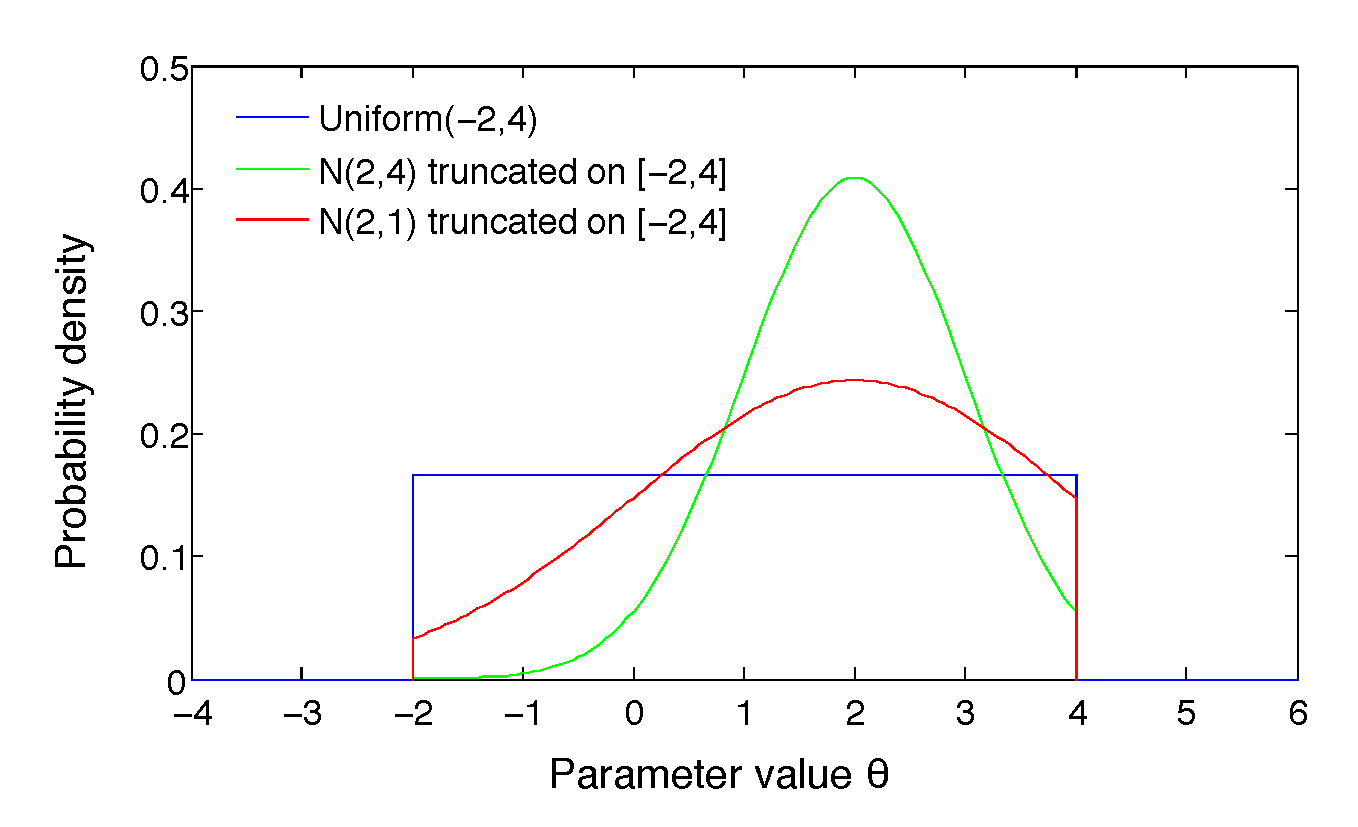
\includegraphics[scale=0.45]{imgs/uniformn.pdf}
\caption{Probability density functions $P(\theta)$ over the interval $[-2,4]$ using a uniform distribution, a truncated normal distribution $\mathcal{N}(2,4)$ and a truncated normal distribution $\mathcal{N}(2,1)$.} 
\label{fig:uniformn}
\end{figure}

\subsection{Instantiation}
\label{sec:rule-params-instantiation}

Parameters are instantiated in the dialogue state as chance nodes.  One distinct node is created for each (univariate or multivariate) parameter distribution and included as a parent of its corresponding rule node. The rule distributions defined in Section \ref{sec:ruleinstantiation} must be slightly adapted to account for these parameters in the parent nodes of the rule.  The rest of the instantiation process remains unchanged. 

\subsubsection*{Parameters of probability rules}

A parametrised probability rule $r$ structured with $n$ conditions is associated with $n$ multivariate parameter nodes $\boldsymbol\theta_{r(1)}, \dots, \boldsymbol\theta_{r(n)}$.  Each distribution $P(\boldsymbol\theta_{r(i)})$ is a Dirichlet distribution of dimension $m_i$, where $m_i$ is the number of effects associated with the condition $c_i$ (including the empty effect). Figure \ref{fig:ruleinstantiation_params} illustrates this instantiation procedure with two probability rules.  

The conditional probability distribution of a rule node $r$ given its input variables $I_1, \dots, I_k$ and parameters $\boldsymbol\theta_{r(1)}, \dots, \boldsymbol\theta_{r(n)}$ is a straightforward adaptation of Equation \eqref{eq:ruledistrib}:
\begin{align}
& P(r\!=\!e \, | \, I_1\!=\!i_1, \dots,  I_k\!=\!i_k\,; \boldsymbol\theta_{r(1)}, \dots, \boldsymbol\theta_{r(n)})  = P(E_i = e\,; \boldsymbol\theta_{r(i)}) \\
& \; \; \; \; \; \; \; \; \text{ where } i = \min_i (c_i \text{ is satisfied with } I_1\!=\!i_1 \land \dots \land I_k\!=\!i_k) \nonumber
\end{align}

The rule distribution in the presence of universally quantified variables defined in Equation \eqref{eq:quantifruledistrib} can be similarly adapted to include parameters.

\subsubsection*{Parameters of utility rules}

The parameters of utility rules are also instantiated as distinct chance nodes in the dialogue state, as shown in Figure \ref{fig:ruleinstantiation_params2}. The corresponding utility distribution is adapted from Equation \eqref{eq:utildistrib} as follows:
\begin{align}
& U_r(D_1'\!=\!d_1, \dots, D_l'\!=\!d_l, I_1\!=\!i_1, \dots, I_k\!=\!i_k\,; \boldsymbol\theta_{r(1)}, \dots, \boldsymbol\theta_{r(n)}) \nonumber \\ 
& = U_i(D_1'\!=\!d_1, \dots, D_l'\!=\!d_l\,; \boldsymbol\theta_{r(i)})  \label{eq:utildistrib_params}\\
& \; \; \; \; \; \; \; \; \text{ where } i = \min_i (c_i \text{ is satisfied with } I_1\!=\!i_1 \land \dots \land I_k\!=\!i_k) \nonumber
\end{align}

\begin{figure}[h!]
\centering
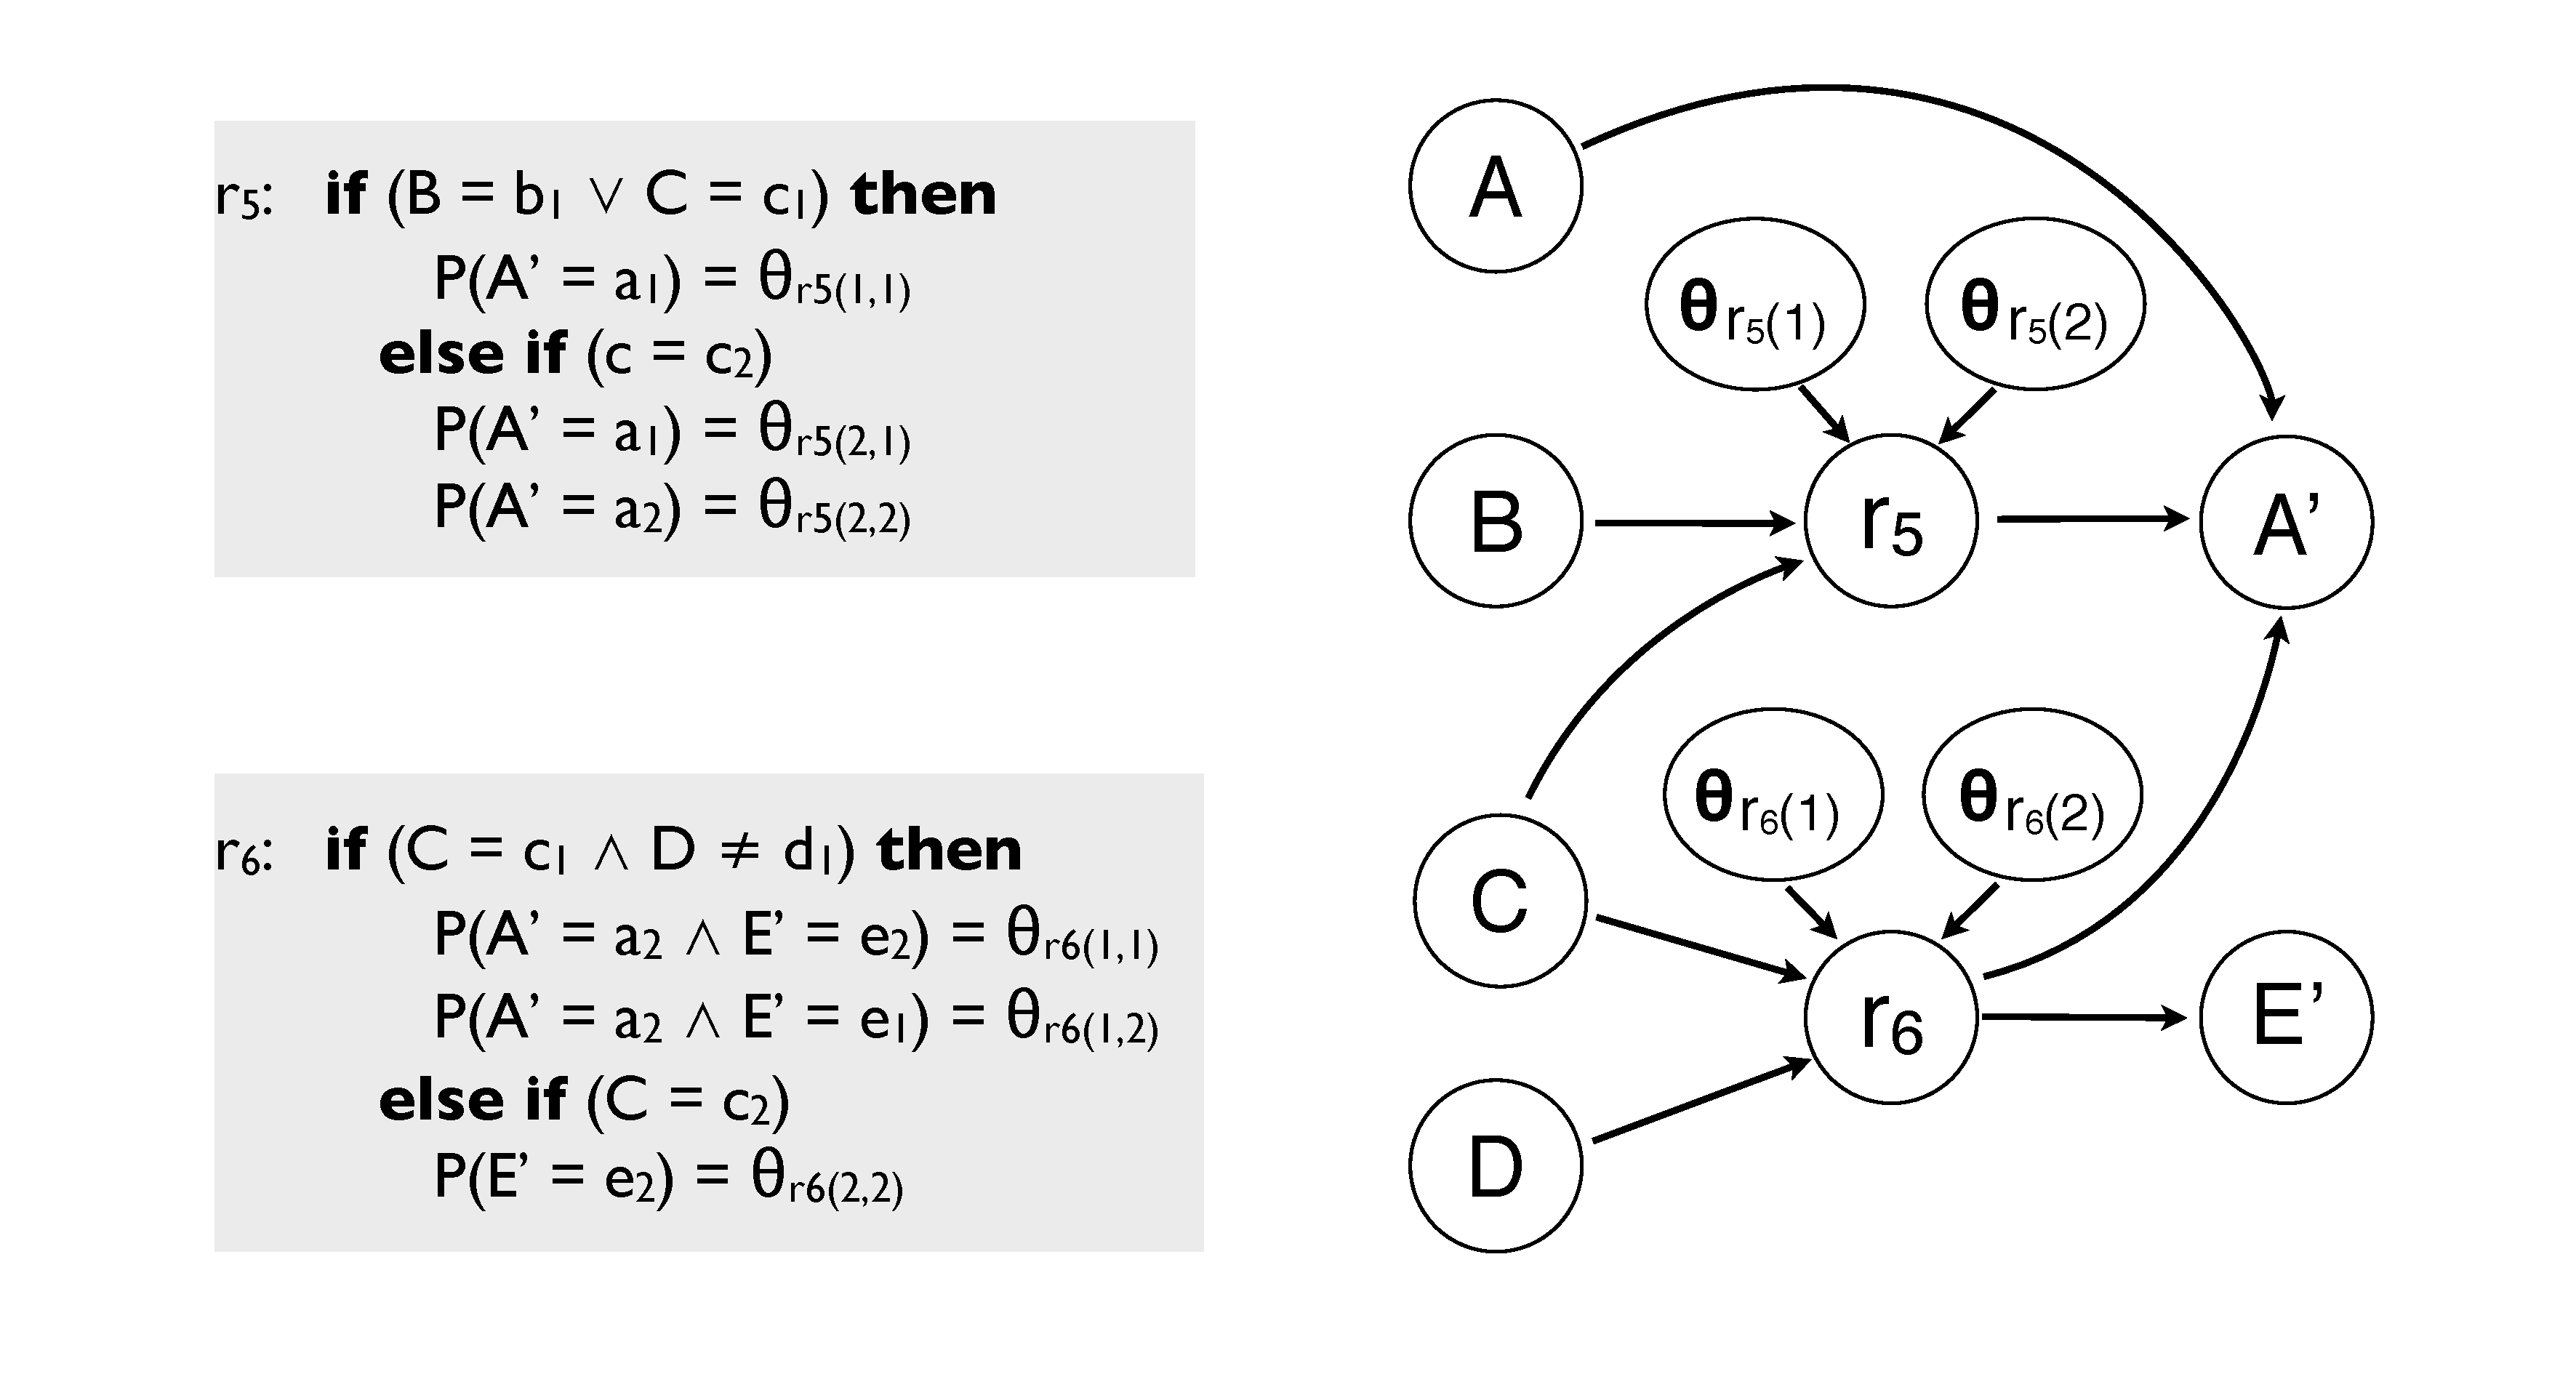
\includegraphics[scale=0.25]{imgs/ruleinstantiation_params.pdf}
\caption{Example of instantiation for two parametrised probability rules $r_5$ and $r_6$.}
\label{fig:ruleinstantiation_params}
\end{figure}


\begin{figure}[h!]
\centering
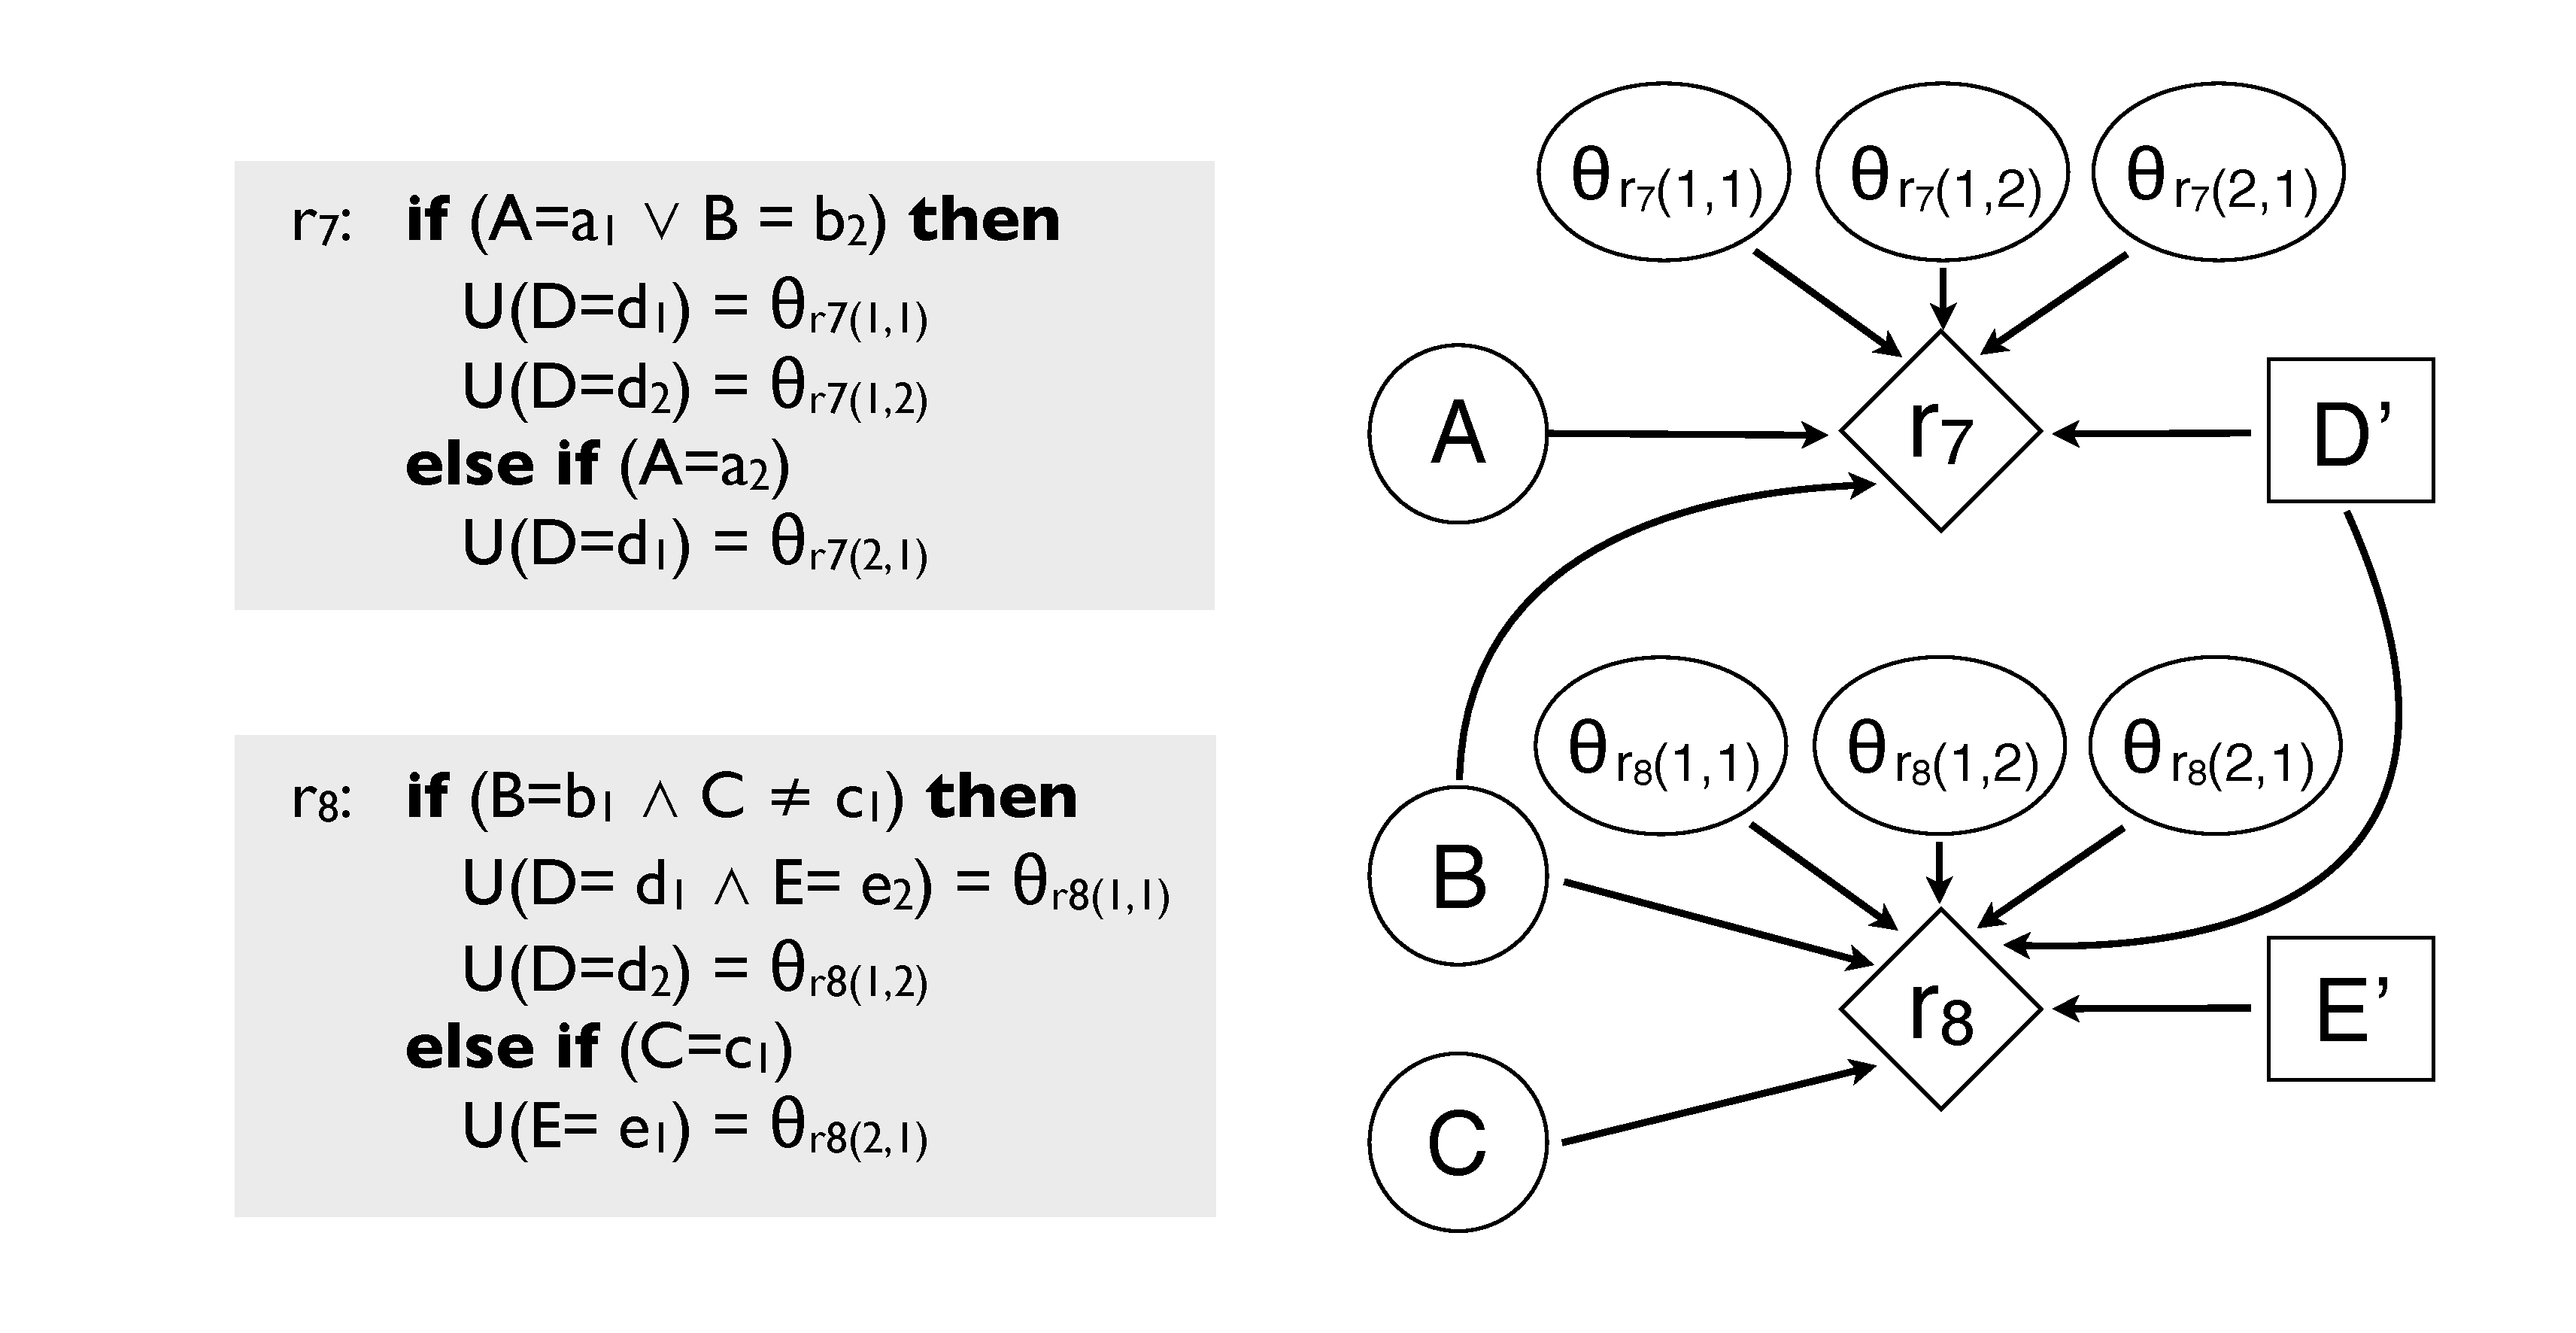
\includegraphics[scale=0.25]{imgs/ruleinstantiation2_params.pdf}
\caption{Example of instantiation for two parametrised utility rules $r_7$ and $r_8$.}
\label{fig:ruleinstantiation_params2}
\end{figure}

\section{Supervised learning of rule parameters}
\label{sec:rule-supervised}
\index{rule parameters!supervised learning of}
\index{supervised learning}

Once the rule parameters are instantiated as nodes in the dialogue state, one can calculate their posterior distribution $P(\boldsymbol\theta \, | \, \mathcal{D})$ after observing a particular data set $\mathcal{D}$ using standard algorithms for probabilistic inference. The estimation of rule parameters corresponds to a learning problem with partial data (cf. Section \ref{sec:learning}), since some of the nodes in the dialogue state  -- such as rule nodes -- are not directly observed. The posterior distribution $P(\boldsymbol\theta \, | \, \mathcal{D})$ is thus no longer guaranteed to remain in the same distribution family as their prior distributions.  The solution adopted here is to approximate the parameter distributions via sampling techniques.
The estimation of rule parameters from data is practically achieved by cycling through the data sample one after the other and gradually refining the parameter distributions in the light of the observed values. We describe in the next pages the generic representation of the training data as well as the learning algorithm employed for the estimation of rule parameters.

\subsection{Wizard-of-Oz training data}
\label{sec:rule-supervised-oz}
\index{Wizard-of-Oz interaction|textbf}

The focus of this chapter is on the estimation of rule parameters from a specific type of training data, namely Wizard-of-Oz interactions. Wizard-of-Oz interactions are interactions between human users and a dialogue system which is remotely controlled by a human expert ``behind the curtains''.  They constitute a simple and efficient method to collect realistic conversational behaviour for a particular domain in the absence of a fully implemented or optimised system. Developing spoken dialogue systems can indeed lead to a ``chicken-and-egg'' dilemma: In order to build up a particular system, system designers often need to know what types of user utterances and behaviours are expected -- but in order to collect such data, one must first have an integrated dialogue system with which the users can interact.  Wizard-of-Oz interactions are a way to circumvent this dilemma.

%We describe below the representation format used to encode these interactions and how domain models can be optimised given some reasonable assumptions about the wizard behaviour. 

\subsubsection*{Representation format}

For the specific purpose of estimating the parameters of dialogue management models, we can represent Wizard-of-Oz interactions as a sequence of state--action pairs $\mathcal{D} = \{\langle \mathcal{B}_i, a_i \rangle : 1 \leq i \leq n\}$, where $\mathcal{B}_i$ corresponds to the dialogue state at time $i$, and $a_i$ is the associated action performed by the wizard.  The number $n$ corresponds to the total number of recorded actions. 
\index{dialogue state}
The dialogue state $\mathcal{B}_i$ represents the current conversational situation at time $i$ as it was perceived by the wizard.  The dialogue state usually includes the recent dialogue history as well as important contextual features.  As explained in the previous chapter, the dialogue state can be encoded as a Bayesian network to reflect state uncertainty and dependencies amongst state variables. Associated to each dialogue state is the corresponding action $a_i$ selected by the wizard at that state. This action can be void if the wizard decides to take no action at that specific step in the dialogue. 

%The sequence of state-action pairs $\mathcal{D}$ is in our approach automatically extracted from the collected interactions, without any manual annotation.  

Many conversational situations allow for multiple, equally ``correct'' system responses.  This characteristic of verbal interactions carries over to the state--action pairs of Wizard-of-Oz data sets, as one can occasionally observe similar states mapped to different wizard actions. The wizard actions should therefore be viewed as an indication of good conversational behaviour, but do not constitute absolute gold standards in the traditional sense of being the uniquely appropriate output for the given dialogue state. The existence of multiple responses also entails that the accuracy of the learned models remains contingent on the degree of internal consistency of the wizard actions. 

\subsubsection*{Assumptions about the wizard behaviour}
\index{Wizard-of-Oz interaction!assumptions about}

The utilities of the system actions are never directly observed -- the only data points available to the learning agent are are the examples of wizard decisions in various situations.  In order to infer the underlying utilities from these examples of decisions, one needs to make a few assumptions about the relation between the action utilities and the decisions made by the wizard. 

Parameter estimation on Wizard-of-Oz data rests on the assumption that the wizard is an (approximately) rational agent and will tend to select actions that are deemed most useful in their respective dialogue state. The agent is only assumed to act rationally \textit{given} the perceived (uncertain) dialogue state. The wizard must indeed act on the basis of ``noisy'' inputs (including e.g.\ speech recognition errors) and may as a consequence select suboptimal actions if the provided inputs contain erroneous hypotheses. It should therefore be stressed that the assumption of rationality does not equate to an assumption of omniscience on the part of the wizard.  Furthermore, in order to account for the occasional errors and inconsistencies in the Wizard-of-Oz data set, the rationality of the wizard decisions is only assumed up to a certain level of confidence (as explained below). 

In practice, the posited rationality of the wizard implies that the likelihood $P_{\mathcal{B}_i}(a_i\,; \boldsymbol\theta)$ of a wizard action $a_i$ in a dialogue state $\mathcal{B}_i$ under the parameters $\boldsymbol\theta$ will depend on the utility of action $a_i$ in $\mathcal{B}_i$ relative to other possible actions.  We now formalise this definition of the likelihood.

\subsection{Learning cycle}
\label{sec:rule-supervised-learning}
\index{supervised learning!as imitation}

The goal of the learning process is to estimate the posterior distribution $P(\boldsymbol\theta \, | \, \mathcal{D})$ over the rule parameters given the collected Wizard-of-Oz data set $\mathcal{D}$. The procedure operates in an incremental fashion by traversing the state--action pairs one by one (in a single pass) and updating the posterior parameter distributions after each pair.  

\subsubsection*{Likelihood distribution}
 \index{likelihood distribution}
One key element of the learning cycle is the definition of the probability $P_{\mathcal{B}_i}(a_i\,; \boldsymbol\theta)$, which specifies the likelihood of the wizard action $a_i$ in a dialogue state $\mathcal{B}_i$ given the parameters $\boldsymbol\theta$. The intuitive purpose of this likelihood is to favour the parameter values that provide a good fit for the wizard action choices. In practice, this is achieved by representing the likelihood of the wizard action $a_i$ in terms of the relative utility of action $a_i$ compared to alternative action choices. The first step is to calculate the utility $U_{\mathcal{B}_i}(a\,; \boldsymbol\theta)$ for all possible actions $a$, and to subsequently rank the actions in descending order of utility.  As the wizard is presupposed to act rationally (modulo a small probability of error), the wizard action is expected to appear at the top of this ranked list of actions. Formally, we express the likelihood of action $a_i$ given the parameters $\boldsymbol\theta$ as:
\begin{align}
P_{\mathcal{B}_i}(a_i\,; \boldsymbol\theta) & = \begin{cases} \eta \, p & \text{if } a_i \ \text{ is the action with highest utility given } \boldsymbol\theta  \\
\eta (1-p) p & \text{ if } a_i \ \text{is the second-highest action} \\
\eta (1-p)^2 p & \text{ if } a_i \ \text{is the third-highest action} \\ 
\dots
\end{cases} \nonumber \\[1mm]
& = \ \ \eta (1-p)^x p \ \ \ \ \ \ \ \text{ where } x \text{ is the position of action } a_i \label{eq:likelihood1} \\[-2mm]
&  \phantom{= (1-p)^x p} \ \ \ \ \ \ \ \ \ \ \ \text{ in the ranked list of actions}  \nonumber
\end{align}

The $\eta$ factor in Eq. \eqref{eq:likelihood1} represents as usual the normalisation factor, while the probability $p$  represents the learner confidence in the rationality  of the wizard.  A value $p = 0.7$ will hence indicate that the wizard is assumed to act rationally -- and thus select the highest-utility action -- with probability $0.7$. The probability $p$ indirectly defines the learning rate of the estimation process: the higher the probability, the faster the learner will converge to a policy that imitates the wizard actions.  However, a high value for $p$ renders the learner more vulnerable to the occasional errors and inconsistencies on the part of the wizard. 


\begin{wrapfigure}[17]{r}{65mm}
\vspace{-2mm}
\centering
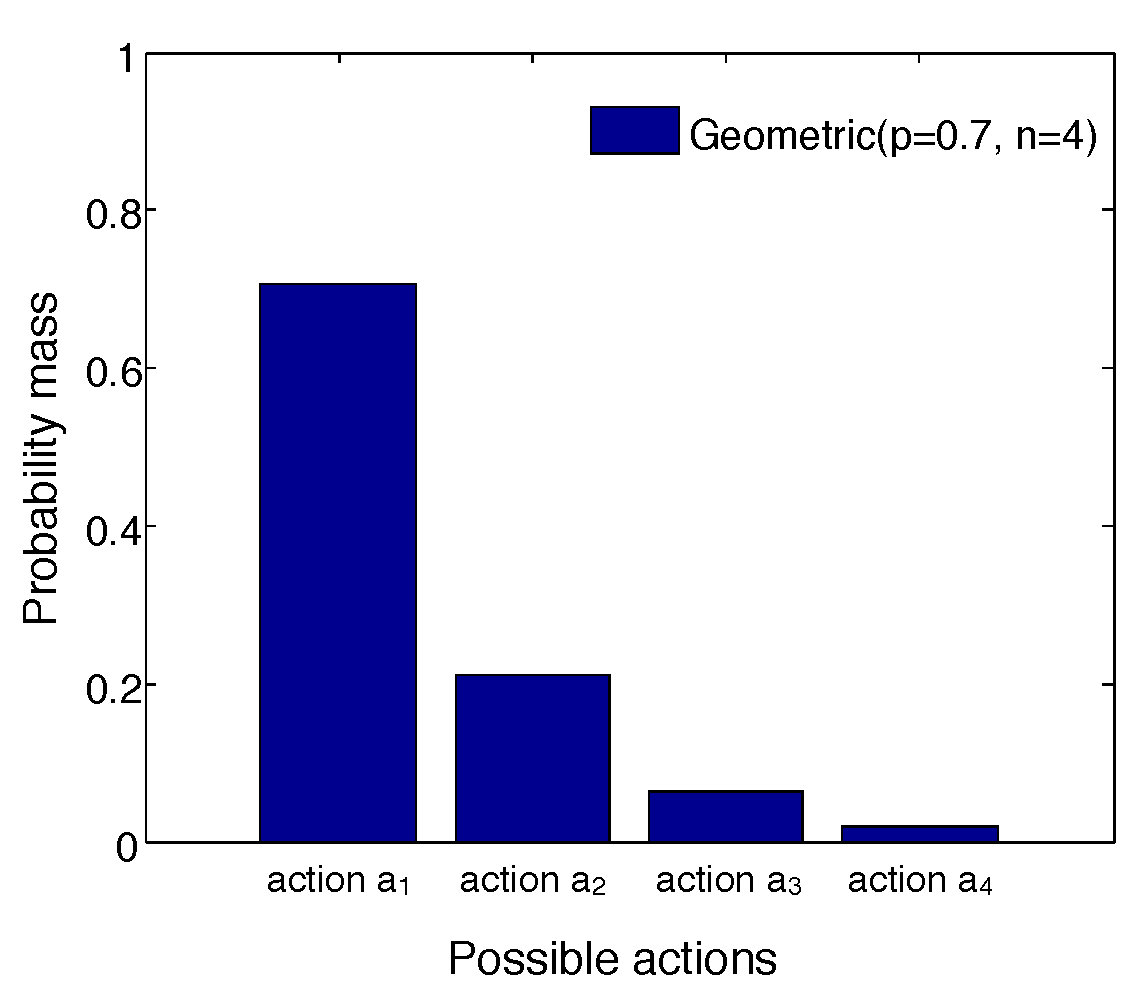
\includegraphics[scale=0.34]{imgs/geometric.pdf} 
\vspace{-6mm}
\caption{Distribution $P_{\mathcal{B}_i}(a_i\,; \boldsymbol\theta)$ for four action values $[a_1, a_2, a_3, a_4]$ ranked by decreasing utility, with $p=0.7$.}
\label{fig:geometric}
\end{wrapfigure}
\index{geometric distribution}
The probability distribution represented by Equation \eqref{eq:likelihood1} is a particular instance of a \textit{geometric} distribution.\footnote{Technically speaking, the definition in Equation \eqref{eq:likelihood1} corresponds to a truncated version of the geometric distribution, as the support of the distribution is finite (the number of possible actions is bounded). The reduction of the distribution to a finite support is achieved via the normalisation factor $\eta$.} Given a repetition of Bernoulli trials with a probability of success $p$, the geometric distribution $\mathrm{Geometric}(p)$  describes the probability that the first success will be observed at the $k$-th trial. 

The reliance on geometric distributions to formalise the likelihood of the observed actions is motivated by the posited rationality of the wizard decisions.  In other words, the formalisation is grounded in the assumption that the wizard will select the highest utility action with probability $p$, the second-highest action with probability $(1-p)p$, and so forth. The geometric distribution is monotonically decreasing, which ensures that the probability of a high-utility action will always be higher than its lower-utility alternatives.   

Figure \ref{fig:geometric} shows an example of geometric distribution over four action values $[a_1, a_2, a_3, a_4]$, where $U_{\mathcal{B}_i}(a_1\,; \boldsymbol\theta) > U_{\mathcal{B}_i}(a_2\,; \boldsymbol\theta) > U_{\mathcal{B}_i}(a_3\,; \boldsymbol\theta) > U_{\mathcal{B}_i}(a_4\,; \boldsymbol\theta)$.


\subsubsection*{Posterior parameter distribution}
\index{posterior distribution}
Given the aforementioned likelihood distribution, the posterior distribution over the parameters is defined via Bayes' rule: 
\begin{equation}
P_{\mathcal{B}_i}(\boldsymbol\theta \, | \, a_i) = \eta \, P_{\mathcal{B}_i}(a_i\,; \boldsymbol\theta) \, P(\boldsymbol\theta ) \label{eq:paramposterior}
\end{equation}

The factor $\eta$ is used for normalisation. The calculation of this posterior distribution is a non-trivial inference problem as the probabilistic model contains both continuous and discrete random variables.  Two types of solutions can be distinguished. \begin{itemize}
\item The first strategy is to discretise the range of parameter values into distinct, mutually exclusive buckets, and thereby transform continuous variables into discrete variables, with a number of values equivalent to the number of buckets employed for the discretisation.
\item The second strategy is to retain the continuous nature of the parameters, but approximate the inference process through the use of sampling techniques.  
\end{itemize}
\index{probability distribution!discretisation of}\index{sampling techniques}
Although both solutions are implemented in the \opendial{} toolkit (see Chapter \ref{chap:opendial}), sampling techniques such as likelihood weighting have in practice proved to be more efficient and scalable than discretisation. 

After sampling, the full joint distribution $P_{\mathcal{B}_i}(\boldsymbol\theta \, | \, a_i)$ is factored into its individual parameter variables. This factorisation corresponds to a simplifying assumption as parameter independence is theoretically no longer guaranteed when handling partially observed data. 
%:\begin{equation}
%P_{\mathcal{B}_i}(\boldsymbol\theta | a_i) = \prod_{\theta_j \in \boldsymbol\theta} P_{\mathcal{B}_i}(\theta_j | a_i)
%\end{equation}

\subsubsection*{Representation of the posterior}

The result of the posterior calculation in Equation \eqref{eq:paramposterior} is a collection of sampled values. In order to derive a full probability density function from these samples, one can either follow a so-called parametric approach and seek to reconstruct the underlying parametric distributions (such as Gaussian or Dirichlet distributions) that best fit the data, or adopt a non-parametric strategy and directly represent the posterior as a function of the collected samples. Parametric approaches, albeit interesting, are difficult to apply in this setting, for two main reasons:
\begin{enumerate}\index{non-parametric distribution}
\item The distribution family of the posterior is hard to determine, as the posterior is no longer ensured to remain in the same family as the prior when learning from partial data.  
\item Additionally, fitting multivariate distributions such as Dirichlets based on sampled values is a laborious computational process with no closed-form solutions.\footnote{Numerical methods based on fixed-point and Newton-Raphson iterations do exist, however \citep{minka2003}.}
\end{enumerate}

We have consequently adopted a non-parametric representation of the posterior distributions, based on \textit{kernel density estimation}\index{kernel density estimation} (KDE).  The kernel density estimator for a continuous variable $X$ for which a set of samples $x_1, \dots, x_n$ is available is given by:
\begin{equation}
P(x) = \frac{1}{nh} \sum_{i=1}^n K\Big(\frac{x-x_i}{h}\Big) \label{eq:kde}
\end{equation}
where $K(\cdot)$ is a \textit{kernel function}\index{kernel function} and $h$ is a smoothing parameter called the \textit{bandwidth}. Multiple kernel functions can be used, but a common choice is to adopt a Gaussian kernel. The kernel density estimator corresponds in this case to a combination of $n$ Gaussians, where each Gaussian is centred on a sample point $x_i$.  This combination of Gaussians is smoothed proportionally to the bandwidth parameter. Figure \ref{fig:kde} illustrates the use of kernel density estimation for a continuous variable based on a set of 50 samples and a Gaussian kernel. The figure shows the influence of the bandwidth parameter on the shape of the resulting density function. Kernel density estimators do not necessitate any particular assumption about the nature of the underlying distribution, and are therefore well-suited to represent distributions of indeterminate type -- as is the case for posterior distributions over the parameters of probabilistic rules. 

\begin{figure}[ht]
\centering
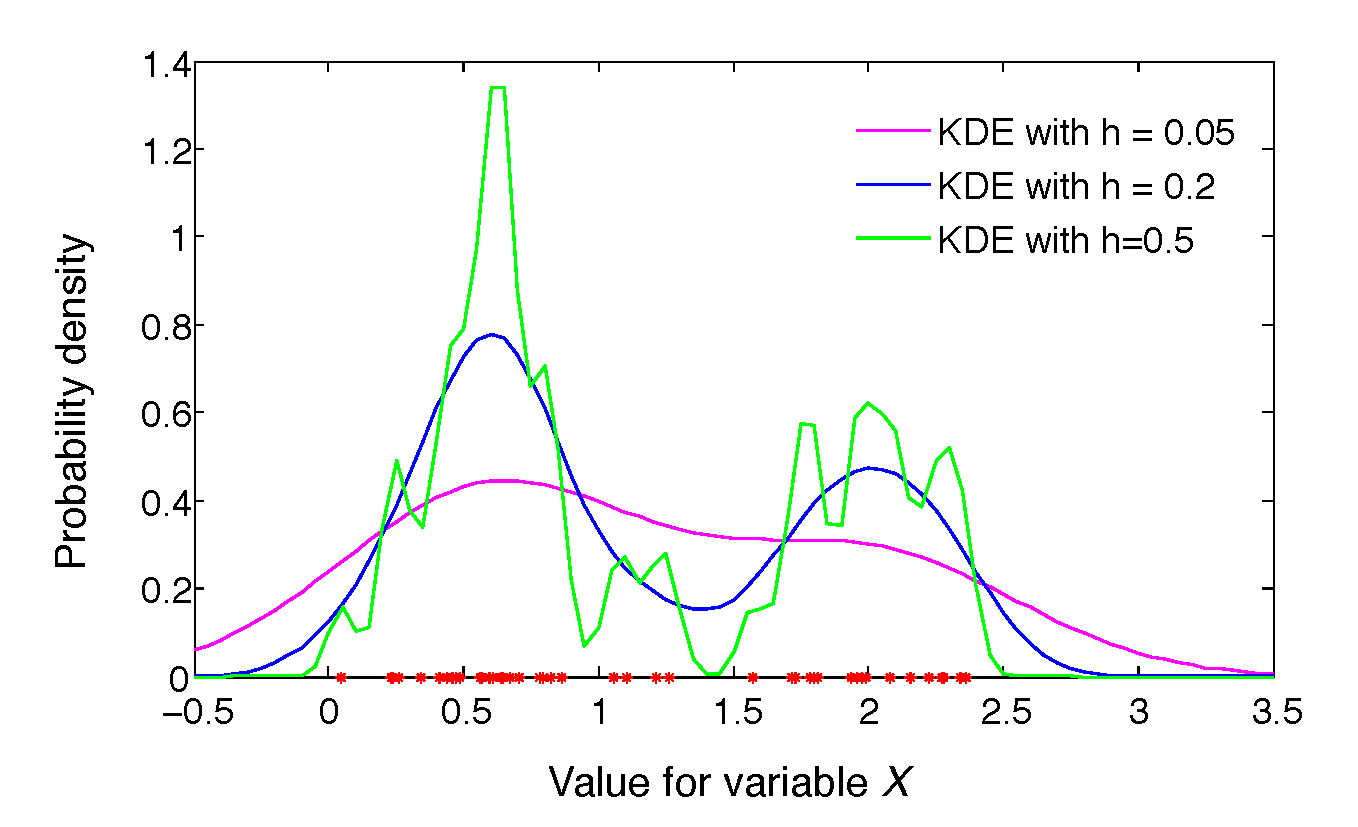
\includegraphics[scale=0.45]{imgs/kde.pdf} 
\caption{Kernel density estimators (KDEs) for a continuous variable $X$ based on 50 samples (shown on the X axis). The density function is shown for three possible bandwidths $h$. }
\label{fig:kde}
\end{figure}

Multivariate distributions are encoded with a multivariate extension of KDE based on product kernels \citep{Silverman1986}.  All estimators in our experiments employ Gaussian kernels with a bandwidth tuned from the sample variance using Silverman's rule of thumb \citep{Silverman1986}. 


\subsubsection*{Learning algorithm}

Algorithm \ref{algo:wozlearning} presents the general procedure for estimating model parameters from Wizard-of-Oz data.  The algorithm loops on each instance pair in the training data.   The posterior parameter distribution is estimated via sampling, based on the likelihood of the wizard action (line 2).  The individual posterior distributions for each parameter are then reconstructed via kernel density estimation on the sampled values (line 3-5), and the process is repeated. 

%For each pair, the algorithm starts by including the parameters in the dialogue state and triggering the domain models (line 2 and 3).

\begin{algorithm}[h!]
\caption{: \textsc{WoZ-learning} ($\mathcal{M}, \boldsymbol\theta, \mathcal{D}, N$)}
\begin{algorithmic}[1] \vspace{1mm}
\REQUIRE Rule-structured models $\mathcal{M}$ for the domain
\REQUIRE Model parameters $\boldsymbol\theta$ with prior distribution $P(\boldsymbol\theta)$
\REQUIRE Wizard-of-Oz data set $\mathcal{D} = \{\langle \mathcal{B}_i, a_i \rangle : 1 \leq i  \leq n\}$
\REQUIRE Number $N$ of samples to draw for each learning example
\ENSURE Posterior distribution $P(\boldsymbol\theta \; | \; \mathcal{D})$ for the parameters  \vspace{1mm}
\FORALL {$\langle \mathcal{B}_i, a_i \rangle \in \mathcal{D}$}
\STATE Set $\mathcal{B}_i \leftarrow \mathcal{B}_i \cup \boldsymbol\theta$
\STATE Trigger models $\mathcal{M}$ on $\mathcal{B}_i$ (cf. Section \ref{sec:processing-workflow})
%\STATE Let $U_{\mathrm{min}}$ be the minimal threshold for the utilities in $\mathcal{B}_i$ \vspace{2mm} 
%\STATE Define likelihood  $P_{\mathcal{B}_i}(a_i\,; \boldsymbol\theta) \leftarrow \dfrac{U_{\mathcal{B}_i}(a_i\,; \boldsymbol\theta) - U_{\mathrm{min}}}{\sum_{a \in \mathit{Val}(A)} \left(U_{\mathcal{B}_i}(a\,; \boldsymbol\theta) - U_{\mathrm{min}}\right)} $ \vspace{2mm} 
\STATE Draw $N$ samples $\mathbf{x}_1, \dots, \mathbf{x}_N$ from posterior $P_{\mathcal{B}_i}(\boldsymbol\theta \, | \, a_i) = \eta \, P_{\mathcal{B}_i}(a_i\,; \boldsymbol\theta) \, P(\boldsymbol\theta )$
\FORALL {parameter variable $\theta \in \boldsymbol\theta$}
\STATE Set $P(\theta) \leftarrow \mathrm{KDE}(\mathbf{x}_1(\theta), \dots, \mathbf{x}_N(\theta))$
\ENDFOR
\ENDFOR
\RETURN $P(\boldsymbol\theta)$
\end{algorithmic}
\label{algo:wozlearning}
\end{algorithm}


\section{Experiments}
\label{sec:wozlearning-experiments}

We evaluated the learning approach outlined in this chapter in the context of a dialogue policy learning task for a human--robot interaction scenario.  The goal of the experiment, originally presented in \cite{rulebasedmodels-sigdial2012}, was to evaluate whether the parameters of a rule-structured utility model could be efficiently optimised from small amounts of Wizard-of-Oz data.  The evaluation metric was defined in this experiment as the proportion of actions corresponding to the wizard selections. The rule-structured model was compared to two baselines encoding the action utilities via traditional representations (plain utility tables and linear functions, respectively). \index{Wizard-of-Oz interaction!agreement measure}

%The empirical results showed that the model encoded with utility rules were able to reproduce the wizard policy  than the more weakly structured baseline models. 

It should be stressed that the purpose of the experiment is limited to the evaluation of the \textit{learning performance}\index{learning performance} of the model. The evaluation of the model in terms of e.g.\ qualitative and quantitative metrics of interaction success (and user satisfaction) constitutes an important but separate question, which will be addressed in Chapter \ref{chap:user-evaluation}. 

We first describe in this section the dialogue domain employed for the experiment, after which we detail the data collection procedure and experimental setup, and finally present and analyse the empirical results. 

\subsection{Dialogue domain}
\label{sec:wozlearning-experiments-domain}
\index{dialogue domain}

The scenario for the Wizard-of-Oz experiment involved a human user and a Nao robot (nicknamed ``Lenny''), which is a programmable humanoid robot developed by Aldebaran Robotics. Figure \ref{fig:nao2} shows a human user interacting with the robot during a data collection experiment. \index{human--robot interaction}\index{Nao robot}

\begin{figure}[ht]
\begin{center}
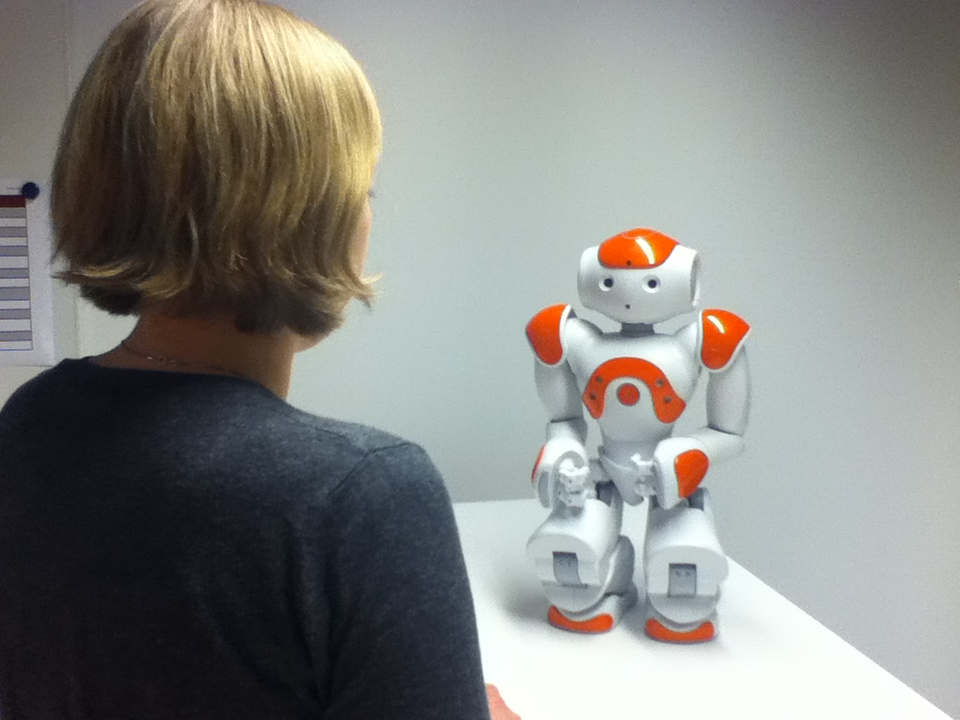
\includegraphics[scale=0.25]{imgs/bilde.jpg}
\end{center}
\caption{Human user interacting with the Nao robot during the Wizard-of-Oz data collection.}
\label{fig:nao2}
\end{figure}

The users were instructed to teach the robot a sequence of body movements such as lifting arms, stepping forward, backward, kneeling down, etc.  The movements could be performed either in consecutive order or in parallel (provided the movements were not in conflict).  The users were free to decide on the movements to perform, and communicated their intention using spoken commands (no gesture recognition was involved).  The robot was programmed to memorise the instructed sequence and could ``replay'' it at any time.

The list of possible dialogue acts\index{dialogue acts} for the user is shown in Table \ref{table:userdas}, and includes a total of 16 dialogue act templates (expanding into 41 dialogue acts when counting all possible argument instantiations). The set of user dialogue acts contains both task-specific dialogue moves to convey user commands as well as conversational actions for feedbacks, acknowledgements, corrections and engagement.  To respond to these user inputs, the robot/wizard had at its disposal a repository of 12 possible actions (expanding into 41 alternative actions when counting all possible instantiations of the action arguments).  The actions included both physical and verbal actions. The verbal actions available to the system comprised various types of clarification requests and grounding acts. The list of system actions is given in Table \ref{table:systemdas}. 

\renewcommand{\arraystretch}{1.3}

\begin{table}[ht]
\begin{footnotesize}
\begin{tabular}{p{60mm}} 
$\cdot$ $\mathrm{MoveArm}(x,y) $ \\ $ \ \ \ \ \ \text{ where } x=\{\mathrm{Left,Right,Both}\} $ \\ $ \ \ \ \ \  \text{ and } y = \{\mathrm{Up,Down,Lateral,}$ \\ $\ \ \ \ \ \ \ \ \ \  \ \ \ \ \ \ \ \ \ \ \ \ \mathrm{Forward,Folded}\}$ \\
$\cdot$ $\mathrm{MoveHead}(y) $ \\ $\ \ \ \ \  \text{ where } y = \{\mathrm{Up,Left,Down,Right}\}$ \\
$\cdot$ $\mathrm{MoveFoot}(x,y) $ \\ $\ \ \ \ \  \text{ where } x = \{\mathrm{Left,Right}\} $ \\ $\ \ \ \ \ \text{ and } y = \{\mathrm{Forward,Backward}\}$ \\
$\cdot$ $\mathrm{Turn}(y) $ \\ $\ \ \ \ \ \text{ where } y = \{\mathrm{Left,Right}\}$ \\ 
$\cdot$ $\mathrm{Kneel}$ \\
$\cdot$ $\mathrm{StandUp}$ 
\end{tabular}
\hspace{2cm}
\begin{tabular}{p{60mm}} 
$\cdot$ $\mathrm{SitDown}$ \\
$\cdot$ $\mathrm{DoMovements}(y) $ \\ $ \ \ \ \ \  \text{ where } y = \{\mathrm{InParallel,InSequence}\}$\\
$\cdot$ $\mathrm{RepeatAll}$ \\
$\cdot$ $\mathrm{ForgetAll}$ \\
$\cdot$ $\mathrm{Confirm}$ \\
$\cdot$ $\mathrm{Disconfirm}$ \\
$\cdot$ $\mathrm{Say}(x)$ \\  $ \ \ \ \ \  \text{ where } x = \{\mathrm{Hello, Compliment,}$ \\ $\ \ \ \ \ \ \ \ \ \ \ \ \ \ \ \ \ \ \ \ \ \ \ \ \  \mathrm{ThankYou, Goodbye}\}$\\
$\cdot$ $\mathrm{GoToInitPose}$ \\ 
$\cdot$ $\mathrm{FollowMe}$ \\
$\cdot$ $\mathrm{Stop}$ 
\end{tabular}
\end{footnotesize}
 \caption{List of user actions $a_u$.} 
\label{table:userdas}
\end{table}

\begin{table}[ht]
\begin{footnotesize}
\begin{tabular}{p{60mm}} 
$\cdot$ $\mathrm{Demonstrate}(z)$ \\ $\ \ \ \ \ \text { where } z = \{\mathrm{MoveArm}(x,y), $ \\ $\ \ \ \ \ \ \ \ \ \ \ \ \ \ \ \ \ \ \ \ \ \ \ \ \  \mathrm{MoveHead}(y),\mathrm{Kneel}, $ \\ $\ \ \ \ \ \ \ \ \ \ \ \ \ \ \ \ \ \ \ \ \ \ \ \ \  \mathrm{StandUp},\mathrm{SitDown}, $ \\ $\ \ \ \ \ \ \ \ \ \ \ \ \ \ \ \ \ \ \ \ \ \ \ \ \  \mathrm{MoveFoot}(x,y), \mathrm{Turn}(y)\}$ \\ $\ \ \ \ \ \text{ and } x, y \text{ take the same values}$ \\ $\ \ \ \ \ \ \ \ \ \ \ \ \ \ \ \ \ \ \ \ \text{as for the user actions}$ \\
$\cdot$ $\mathrm{Say}(x)$ \\  $ \ \ \ \ \  \text{ where } x = \{\mathrm{Hello, ThankYou,}$ \\ $\ \ \ \ \ \ \ \ \ \ \ \ \ \ \ \ \ \ \ \ \ \ \ \ \  \mathrm{Goodbye}\}$
\end{tabular}
\hspace{2cm}
\begin{tabular}{p{60mm}} 
$\cdot$ $\mathrm{AskConfirmation}$ \\
$\cdot$ $\mathrm{RegisterMove}$ \\
$\cdot$ $\mathrm{UndoMove}$ \\
$\cdot$ $\mathrm{AskRepeat}$ \\
$\cdot$ $\mathrm{Acknowledgement}$ \\
$\cdot$ $\mathrm{AskIntention}$ \\
$\cdot$ $\mathrm{DemonstrateAll}$ \\
$\cdot$ $\mathrm{ForgetAll}$ \\
$\cdot$ $\mathrm{StopMove}$ \\
$\cdot$ $\mathrm{FollowUser}$ 

\end{tabular}
\end{footnotesize}
\caption{List of system actions $a_m$.} 
\label{table:systemdas}
\end{table}

\subsection{Wizard-of-Oz data collection}
\label{sec:wozlearning-experiments-woz}

\subsubsection*{System architecture}
\index{dialogue system architecture}

An integrated dialogue system was developed to collect Wizard-of-Oz interactions for the human--robot interaction domain described above. The dialogue system used to collect the Wizard-of-Oz data is equipped with all standard processing modules for speech understanding, generation and robot control.  Figure \ref{fig:exp1_architecture} illustrates the general system architecture and its connection to the robotic platform. At the centre of the architecture lies a shared dialogue state to which multiple system components are attached. These components monitor the dialogue state for relevant changes and read/write to it as they process their data flow. The dialogue manager is replaced by the wizard during data collection. 

\begin{figure}[ht]
\begin{center}
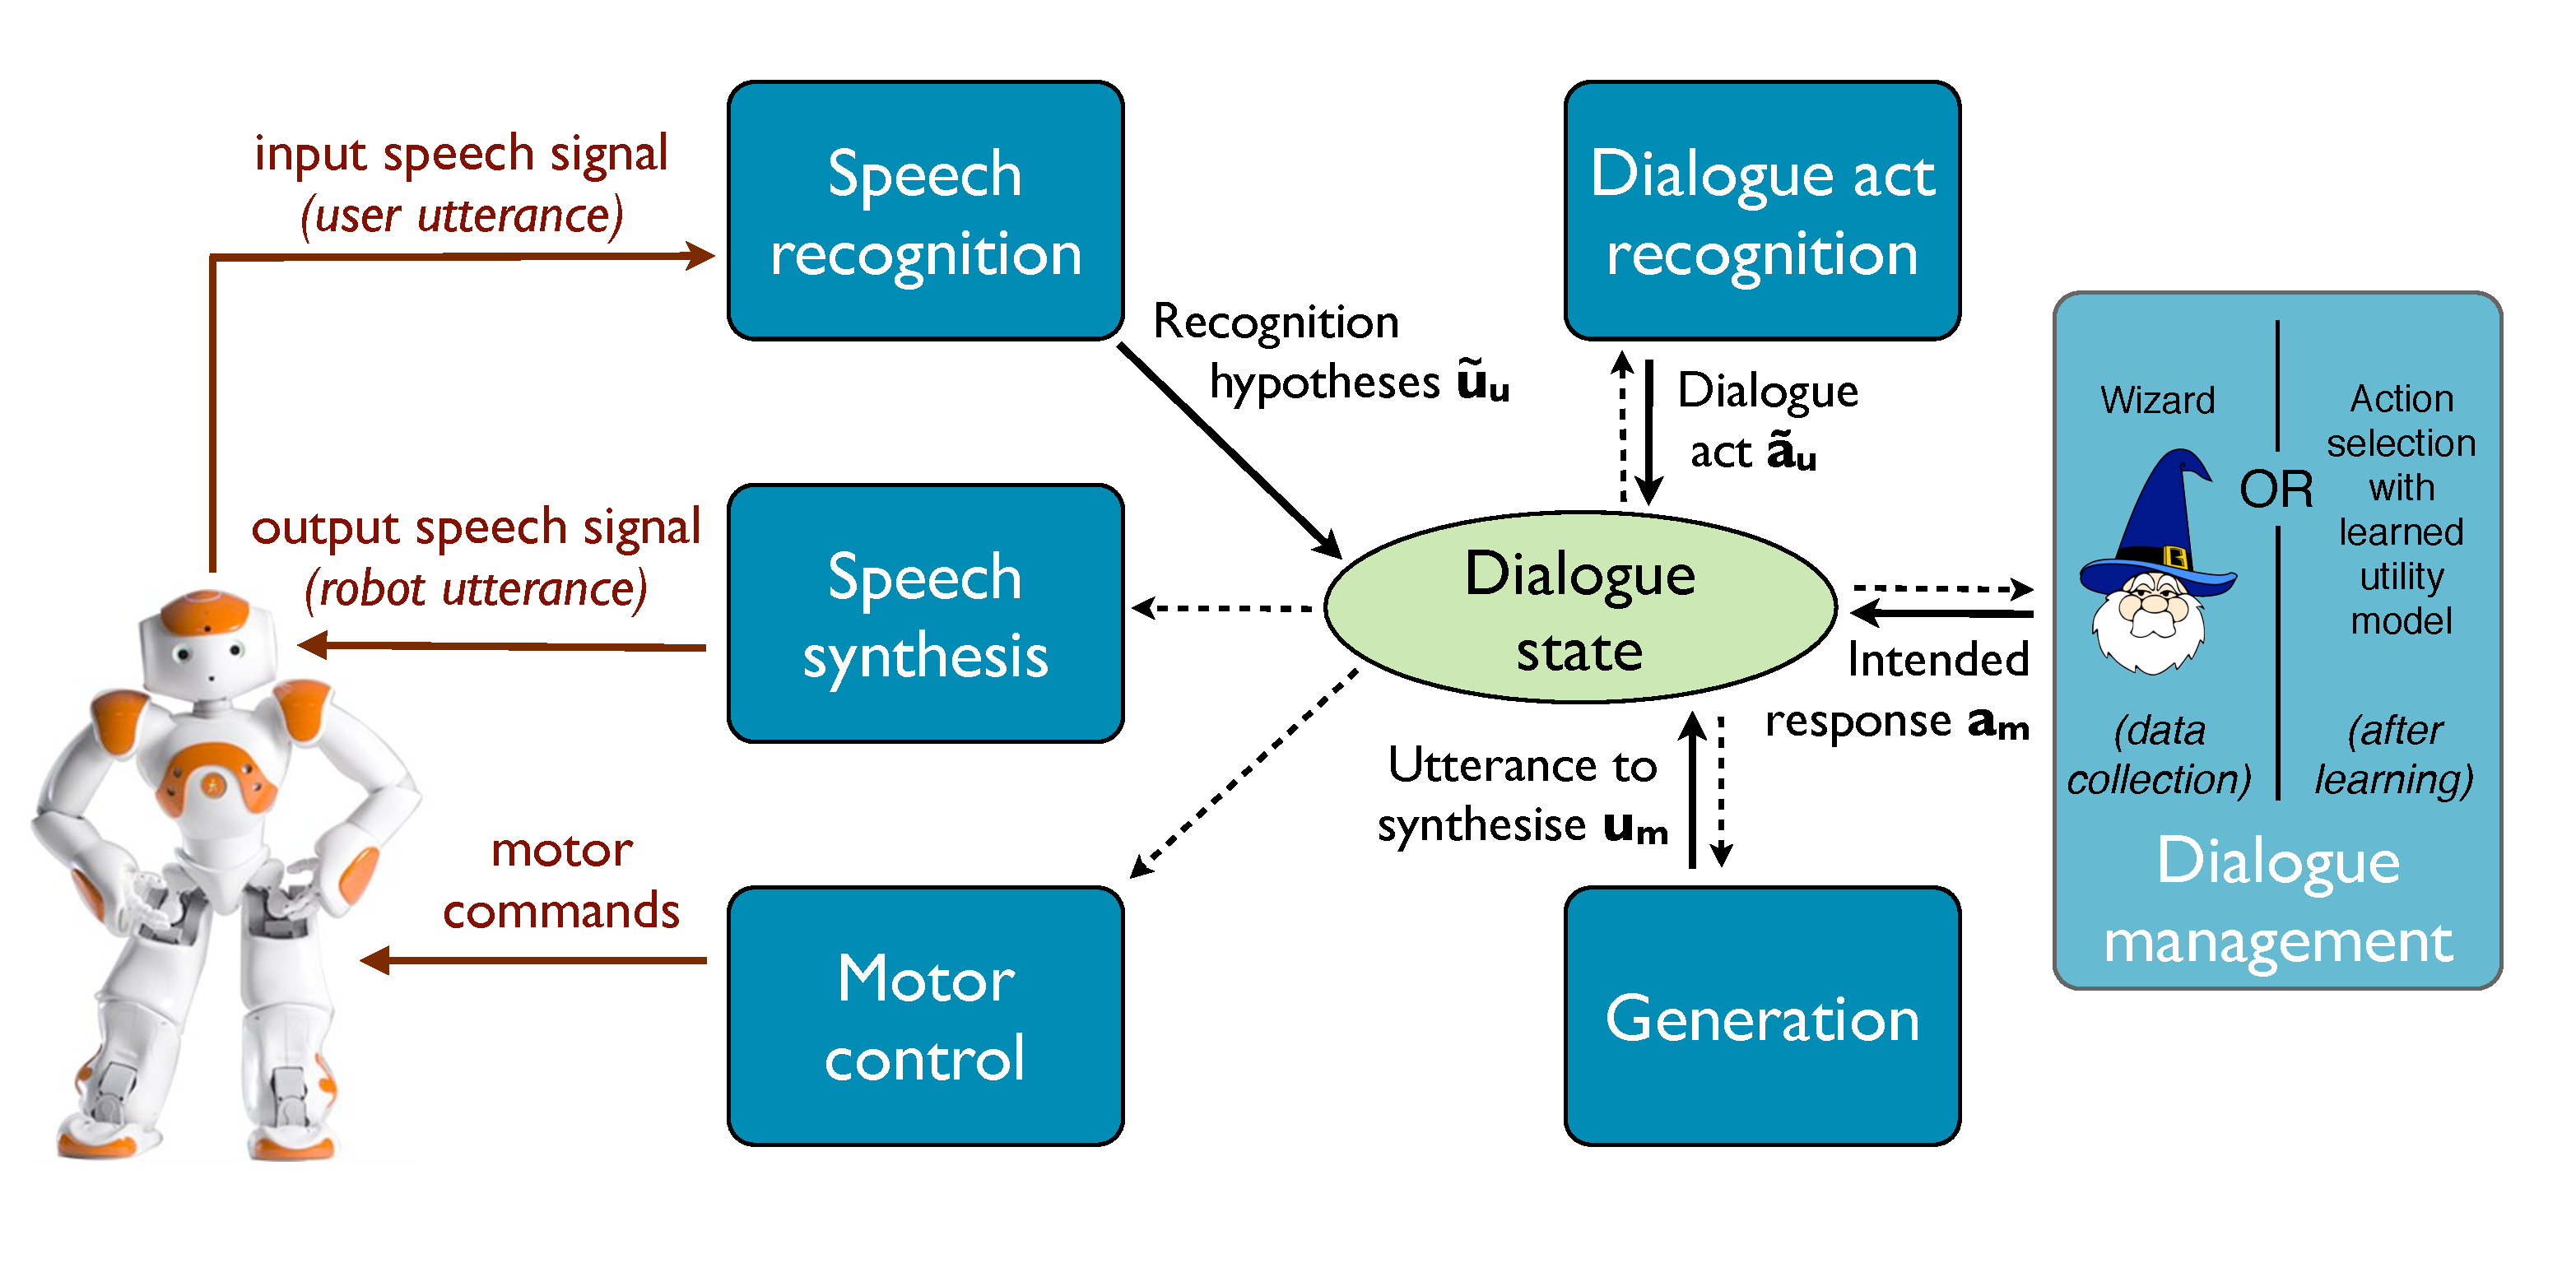
\includegraphics[scale=0.30]{imgs/exp1_architecture.pdf}
\end{center}
\caption{System architecture used for the experiment.}
\label{fig:exp1_architecture}
\end{figure}

The modules used for the experiments include in particular an off-the-shelf speech recogniser connected to four microphones placed on the robot head. The language model of the speech recogniser is encoded with a small hand-crafted recognition grammar. The corresponding user dialogue acts are then derived from the ASR hypotheses via a template-based recognition model. On the generation side, a shallow generation model is in charge of the linguistic realisation of the verbal actions which is then sent to the speech synthesis engine.  Finally, the execution of physical actions is delegated to a separate component, responsible for planning the robot movements and controlling its motors in real-time.  Chapter \ref{chap:opendial} discusses the design choices involved in the development of the dialogue system.

\subsubsection*{Data collection procedure}
\index{Wizard-of-Oz interaction!data collection}
 Each recorded dialogue involved one human subject interacting with the Nao robot in a shared visual scene.  The dialogues were relatively short, with an average duration of about four minutes. We collected a total of 20 interactions with 7 distinct users, for a total of 1020 system turns, summing to around one hour of interaction.  The users were recruited amongst students and researchers in the Department of Informatics at the University of Oslo, while the role of the wizard was taken by the author of the present thesis.  All the interactions were performed in English. All but one user were non-native speakers of English.\footnote{This mismatch between the acoustic model trained on native U.S. English data and the foreign accents of the participants may partly explain the relatively high level of speech recognition errors.}  As the speech recogniser relied on a language model of limited coverage, the users were briefed before each experiment about the comprehension capabilities of the robot in order to adjust their expectations about what the robot could and could not understand, and thereby limit the number of out-of-coverage utterances.

Wizard-of-Oz experiments should ideally place the wizard in the same types of decision contexts as the ones encountered by the dialogue manager. To this end, the wizard was prevented from listening directly to the spoken utterances of the user and was instead provided with the N-best list generated by the speech recogniser.  The N-best lists appeared on the control screen of the wizard as hypotheses accompanied with their respective probabilities. On the basis of these inputs, the wizard could then select the action to perform from a list of alternatives.  

Transcripts 1 and 2 present two recorded excerpts of Wizard-of-Oz interactions.  The user utterances are displayed as N-best lists of speech recognition hypotheses. 

\begin{Transcript}[p!]
\begin{dialogue} \vspace{3mm}
\speak{Human} $\begin{bmatrix}\text{ hello Lenny} & 0.22 \\
\text{ follow me} & 0.20 \\
\text{ hi Lenny} & 0.53 \end{bmatrix}$ \vspace{3mm}
\speak{Robot} \ \ \ Hello there!\vspace{3mm}
\speak{Human} $\begin{bmatrix}\text{ move your left arm up} & 0.41 \\
\text{ move the left arm up} & 0.27 \\
\text{ put your left arm up} & 0.30 \end{bmatrix}$ \vspace{3mm}
\speak{Robot} \ \ \ Sure! \vspace{2mm}\\
\direct{\refer{Robot} executes the movement $\mathrm{MoveArm(Left,Up)}$} \\
\direct{\refer{Robot} waits a few seconds} \vspace{2mm}
\speak{Robot} \ \ \ Was that correct? \vspace{3mm}
\speak{Human} $\begin{bmatrix}\text{ yes} & 0.88 \\
\text{ thanks} & 0.10 \end{bmatrix}$ \vspace{2mm} \\
\direct{\refer{Robot} registers the movement as confirmed} \vspace{3mm}
\speak{Robot} \ \ \ Great \vspace{3mm}
\speak{Human} $\begin{bmatrix}\text{ move your right arm up at the same time} & 0.26 \\
\text{ put the right arm up at the same time} & 0.32 \\
\text{  move the right arm up at the same time} & 0.38 \end{bmatrix}$ \vspace{3mm}
\speak{Robot} \ \ \ Let's see \vspace{1mm} \\
\direct{\refer{Robot} executes movement $\mathrm{MoveArm(Both,Up)}$} \vspace{2mm}
\speak{Robot} \ \ \ Was that correct? \vspace{3mm}
\speak{Human} $\begin{bmatrix}\text{ kneel} & 0.25 \\
\text{ thanks} & 0.14 \\
\text{  no} & 0.57 \end{bmatrix}$  \vspace{2mm} \\
\direct{\refer{Robot} discards last movement and goes back to previous position} \vspace{2mm}
\speak{Robot} \ \ \ What should I do then?  \\
\end{dialogue}
\vspace{-4mm} \hspace{1cm}\direct{...} \vspace{3mm}
\caption{User interaction with wizard-controlled robot, first excerpt}
\end{Transcript}

\begin{Transcript}[p!]
\vspace{4mm} \hspace{1cm} \direct{...}
\begin{dialogue} 
\speak{Human} $\begin{bmatrix}\text{ stop} & 0.25 \\
\text{ stand up} & 0.41 \\
\text{ no} & 0.25 \end{bmatrix}$ \vspace{3mm}
\speak{Robot} Let's see \vspace{1mm} \\
\direct{\refer{Robot} executes movement $\mathrm{StandUp}$} \vspace{3mm}
\speak{Human}  $\begin{bmatrix}\text{ put your right arm forward} & 0.31 \\
\text{ move your right arm forward} & 0.36 \\
\text{ move the right arm forward} & 0.30 \end{bmatrix}$ \vspace{2mm} \\
\speak{Robot} Let's see \vspace{1mm} \\
\direct{\refer{Robot} registers movement $\mathrm{StandUp}$ as implicitly confirmed} \\
\direct{\refer{Robot} executes movement $\mathrm{MoveArm(Right,Forward)}$} \vspace{3mm}
\speak{Human} $\begin{bmatrix}\text{ move forward the left arm} & 0.31 \\
\text{ lower the left arm} & 0.35 \\
\text{ lower both arms} & 0.29 \end{bmatrix}$ \vspace{3mm}
\speak{Robot} Sorry, could you repeat? \vspace{3mm}
\speak{Human} $\begin{bmatrix}\text{ raise your left arm} & 0.28 \\
\text{ lift your right arm} & 0.31 \\
\text{ lift your left arm} & 0.37 \end{bmatrix}$ \vspace{3mm}
\speak{Robot} Sure \vspace{1mm} \\
\direct{\refer{Robot} executes movement $\mathrm{MoveArm(Left,Up)}$} \\
\direct{\refer{Robot} waits a few seconds} \vspace{3mm}
\speak{Robot} Should I do it like this? \\
\speak{Human} $\begin{bmatrix}\text{ kneel} & 0.23 \\
\text{ wrong} & 0.22 \\
\text{ no} & 0.47 \end{bmatrix}$ \vspace{3mm} \\
\direct{\refer{Robot} discards last movement and goes back to previous position} \vspace{2mm}
\speak{Robot} What should I do then?  \vspace{3mm}
\speak{Human} $\begin{bmatrix}\text{ move your left arm up} & 0.29 \\
\text{ move the left arm up} & 0.34 \\
\text{ move the left arm down} & 0.28 \end{bmatrix}$ \vspace{3mm} \\
\end{dialogue}
\vspace{-4mm} \hspace{1cm} \direct{...} \vspace{3mm}
\caption{User interaction with wizard-controlled robot, second excerpt}
\end{Transcript}

\subsubsection*{Dialogue state}
\index{dialogue state}
Each selected action $a_m$ was recorded along with the complete dialogue state $\mathcal{B}$ in effect at the time of the selection. The dialogue state consisted of five independent variables: \begin{enumerate}
\item The last user dialogue act $a_u$ (with the values given in Table \ref{table:userdas})
\item The last system action $a_m$ (with the values given in Table \ref{table:systemdas})
\item The recorded sequence of (confirmed) movements, encoded as a list
\item The last physical movement demonstrated by the robot
\item Finally, a periodically updated variable expressing the number of seconds elapsed since the last user or system action.  This variable is used to determine when the system should ask for an explicit confirmation from the user.
\end{enumerate}

The state variables are represented with their full probability distributions. The dialogue state recorded right before the wizard registers the first movement in Transcript 1 corresponds for instance to the following specification: 
\begin{align*}
\mathcal{B} = \begin{cases} a_u = [ (\mathrm{Confirm}, p\!=\!0.88), (\mathrm{Say(ThankYou)}, p\!=\!0.10), (\mathit{None}, p\!=\!0.02) \rangle \\
a_m = \langle (\mathrm{AskConfirmation}, p\!=\!1) ] \\
\mathit{moveSequence} = [ ( \emptyset, p\!=\!1) ] \\
\mathit{lastMove} = [ (\mathrm{MoveArm(Left,Up)}, p\!=\!1) ] \\
\mathit{silence} = [ (2 \textrm{ seconds}, p\!=\!1) ] \end{cases}
\end{align*}

\subsection{Experimental setup}
\label{sec:wozlearning-experiments-setup}

The central question investigated in this experiment is the following: Does the encoding of dialogue management models in terms of probabilistic rules improve the efficiency of the parameter estimation process compared to more traditional representations? If yes, how significant is the difference? The experiment focused therefore on the learning performance of various utility models based on limited amounts of training data gathered from Wizard-of-Oz interactions. The parameters correspond here to the utilities of the various system actions depending on the current state.

\subsubsection*{Baseline models}

The experiment relied on two distinct baselines that express the utility model of the domain based on traditional representations: \begin{enumerate}
\item The first baseline is a plain utility table\index{utility table} that maps every combination of state values and actions to a particular utility.  For a given set of state variables $X_1, \dots, X_n$, 
the utility for the system action $a_m'$ is therefore defined by: 
\begin{equation}
U(X_1=x_1, \dots, X_n=x_n, a_m') = \theta_{(x_1, \dots, x_n, a_m')}
\end{equation}
where the $\theta_{(x_1, \dots, x_n, a_m')}$ value corresponds to the utility encoded in the table for the state--action pair. The number of required parameters is thus $|\mathit{Val}(X_1)| \times \dots \times |\mathit{Val}(X_n)| \times |\mathit{Val}(a_m')|$. In order to keep the model tractable, the utility table was factored in the experiments in three parts, each responsible for a subset of the possible system actions. These utility tables comprised a total of 8962 independent parameters. 
%\begin{align*}
%&U(a_u,a_m',\mathit{lastMove},\mathit{moveSequence},\mathit{silence},a_{m}') \\ 
%&= U(a_u, a_m',a_{m}') + U(a_u,\mathit{lastMove},a_{m}') + U(a_m',\mathit{silence},a_{m}') 
%\end{align*}
\item The second baseline defines the utility of a given action as a linear combination\index{linear model} of values -- one for each state variable.  The total utility is thus determined as:
\begin{equation}
U(X_1=x_1, \dots, X_n=x_n, a_m') = \sum_{i=1}^{n} \theta_{(x_i, a_m')}
\end{equation}
where $\theta_{(x_i, a_m')}$ corresponds to the utility weight of the variable value $x_i$ for the action $a_m'$.  Note that the weights are specific to a given action value. The number of required parameters is here $|\mathit{Val}(a_m')| \times (|\mathit{Val}(X_1)| + \dots + |\mathit{Val}(X_n)|)$.  As a consequence, the size of the linear model is reduced to 581 independent parameters.  However, this baseline hinges on the assumption that the total utility of a given action can be decomposed as a linear combination of weights for each state variable value.
\end{enumerate}

\subsubsection*{Rule-structured model}
\index{rule-structured model}
The two baselines were compared to a utility model structured with 15 utility rules. The interested reader is invited to browse the specification of these rules in Appendix \ref{chap:domainspecs} (Section \ref{sec:domainspecs-wozlearning}) . The rule structure was designed by hand, while the parameters (in this case, utility values) remained unknown. The rules were associated with a total of 24 parameters. 

\subsubsection*{Parameter estimation}
\index{parameter estimation}

Figure \ref{fig:exp1_baselines} offers a graphical comparison of the utility models produced for the two baselines and the rule-structured approach.  The two baselines are essentially ``flattened'' or unstructured versions of the rule-based model.  The input and output variables remain identical in all three models. However, the two baselines directly associate each state--action combination to a single utility value, while the rule-structured approach defines this overall utility in a more indirect manner, through the instantiation of multiple utility rules. 

\begin{figure}[ht]
\centering
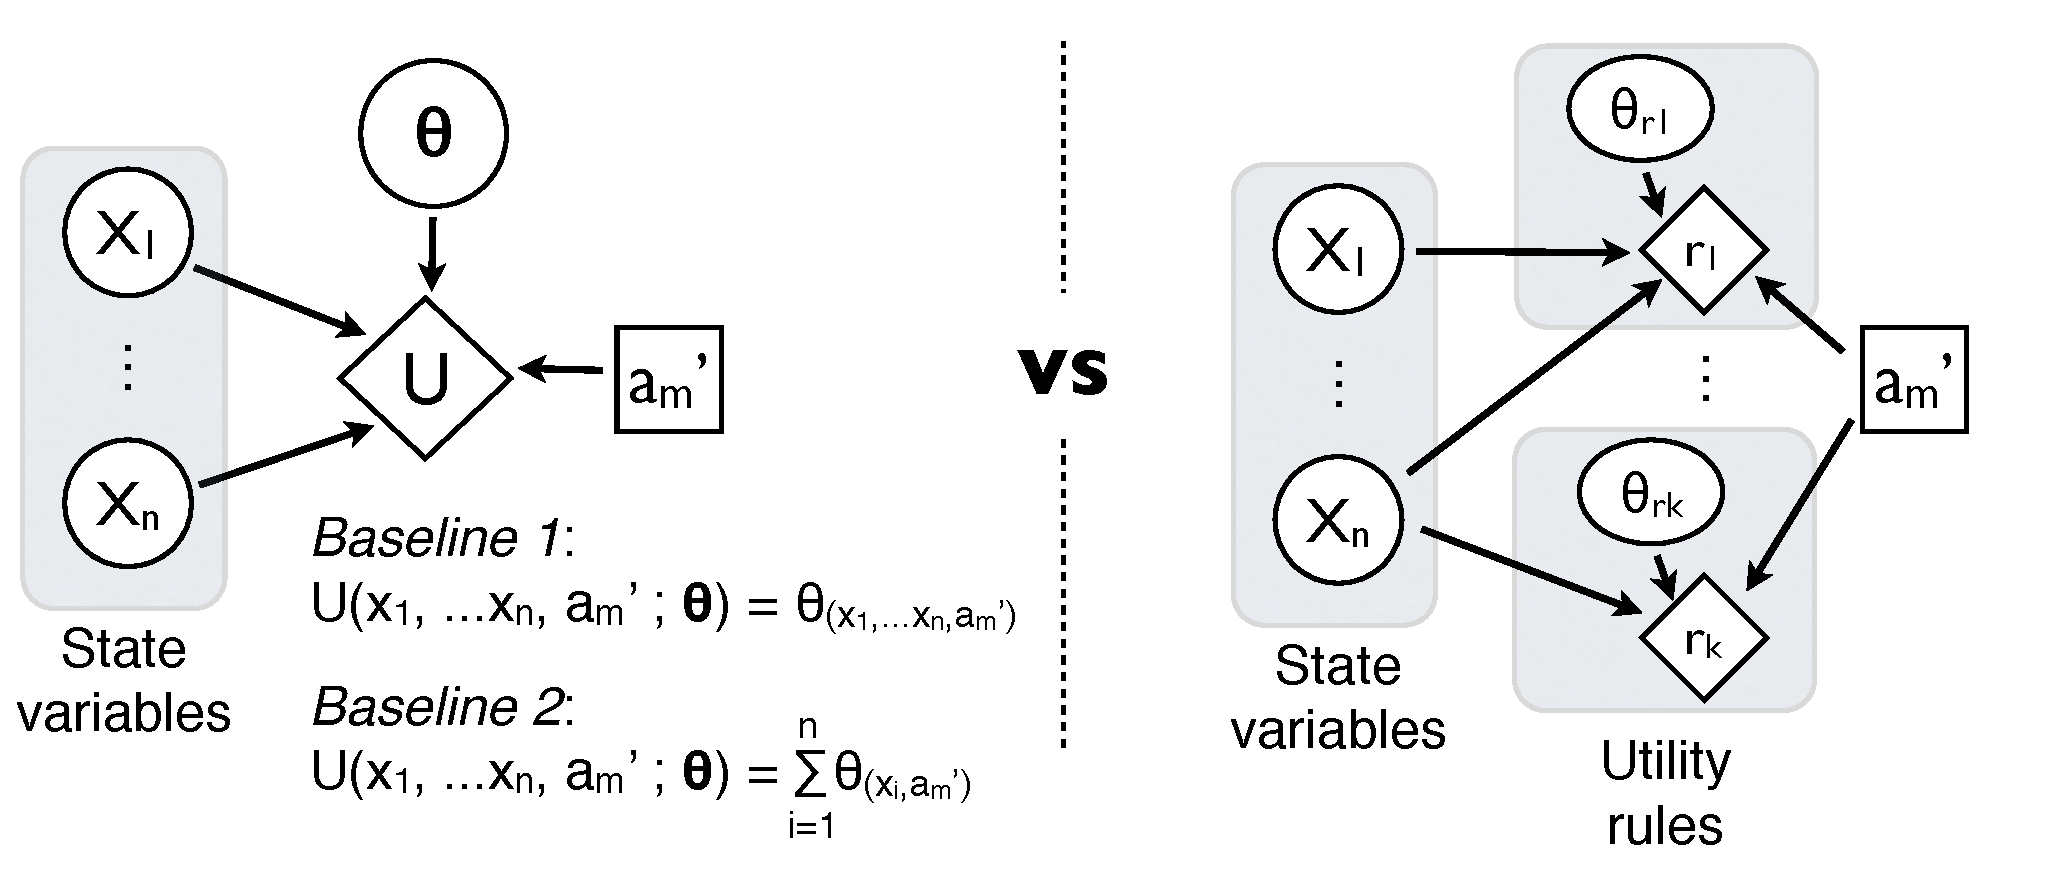
\includegraphics[scale=0.40]{imgs/exp1_baselines.pdf}
\caption{Baseline utility models (left) compared to the rule-structured utility model (right).}
\label{fig:exp1_baselines}
\end{figure}


The parameter estimation procedure followed the Bayesian learning approach detailed in Section \ref{sec:rule-supervised-learning}.  The prior distributions on the utility values were initialised with uniform priors on the interval $[-1,6]$ in all three models. 

%For the baseline models, the function \textsc{triggerModels}(...) resulted in the creation of one single utility node connected to the system action, as illustrated in Figure \ref{fig:exp1_baselines}.

\subsubsection*{Evaluation of learning performance}
\index{learning performance}
Given the utility models defined above, the selected action simply corresponds to the action associated with the maximum utility in the current state. In this particular experiment, utility maximisation only considered the current (immediate) utility and did not perform forward planning.

The data collected from the Wizard-of-Oz interactions was split into a training set composed of 765 state--action pairs (75 \% of the gathered data) and a held-out test set with 255 actions (remaining 25 \%). The same training set was used to estimate the utility parameters for the three models.  The resulting utility models were then evaluated on the basis of their agreement with the wizard actions in the held-out test set. This agreement is determined to be the proportion of system-selected actions that are identical to the action chosen by the wizard. The agreement results for the three models were evaluated at various stages of the estimation process in order to analyse and compare their learning performance. The results were practically calculated by sampling over the parameters, performing inference over the resulting models, and finally averaging over the inference results.  

\subsection{Empirical results and analysis}
\label{sec:wozlearning-experiments-results}

Table \ref{table} presents the agreement results for the three utility models. The differences between the rule-structured model and the two baselines are statistically significant using Bonferroni-corrected paired $t$-tests, with $p$-value $< 0.0001$.   

We performed an error analysis on the 17\% of actions that deviate from the wizard behaviour.\footnote{One should be wary of labelling these actions as ``incorrect'', since they are in most cases relevant dialogue moves, but simply result from slightly different decision strategies than the one followed by the wizard.} The analysis revealed that the discrepancy is mainly due to two factors.  The first factor is the lack of complete consistency on the part of the wizard, who occasionally decided to follow different strategies in similar situations (especially regarding the use of clarification requests). The second factor is the presence of a non-negligible number of spurious and noisy data points, notably caused by interruptions and technical issues with the robotic platform (e.g.\ movements that had to be repeated due to motor failures).

\begin{table}[ht]
\begin{center}
\begin{tabular}{|l|c|} \hline
\textit{Type of model} & \textit{Agreement (in \%) } \\ \hline \hline
Plain utility table & 67.35 \\ \hline
Linear model & 61.85 \\ \hline
Rule-structured model & \textbf{82.82} \\ \hline
\end{tabular}
\end{center}
\vspace{-2mm}
\caption{Agreement results for the three models on a held-out test set.}
\vspace{-2mm}
\label{table}
\end{table}

The learning curves for the three models are shown in Figure \ref{results}\index{learning curve}.   Note that since the parameters are initially uniformly distributed, the agreement is already non-zero before learning, since a random assignment of parameters has a low but non-zero chance of leading to the right action. 


\begin{figure*}[p!]
\begin{center}\subfigure[Linear scale]{
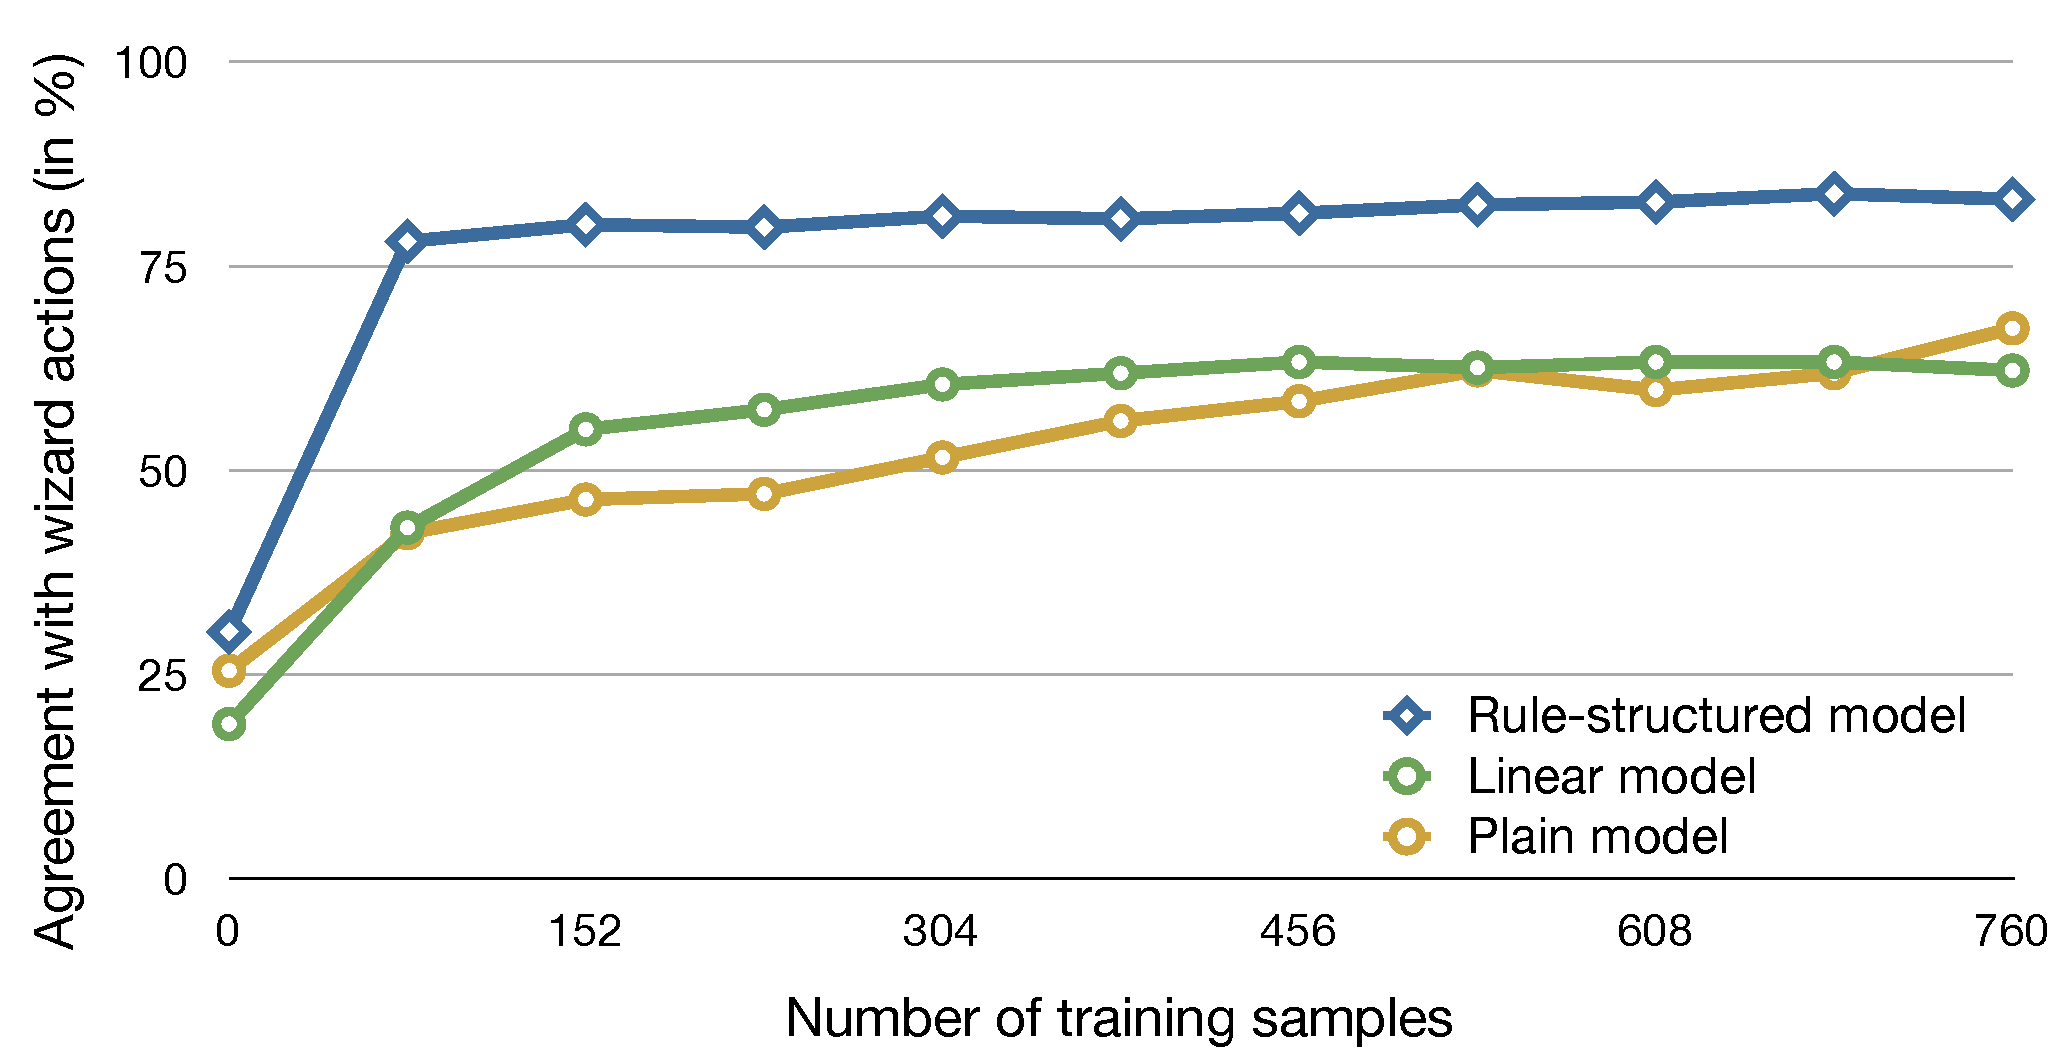
\includegraphics[scale=0.38]{imgs/results_linear.pdf}
}\end{center} $\phantom{a}$\vspace{8mm}$\phantom{a}$ 
\begin{center}\subfigure[Logarithmic scale (base 2)]{
\centering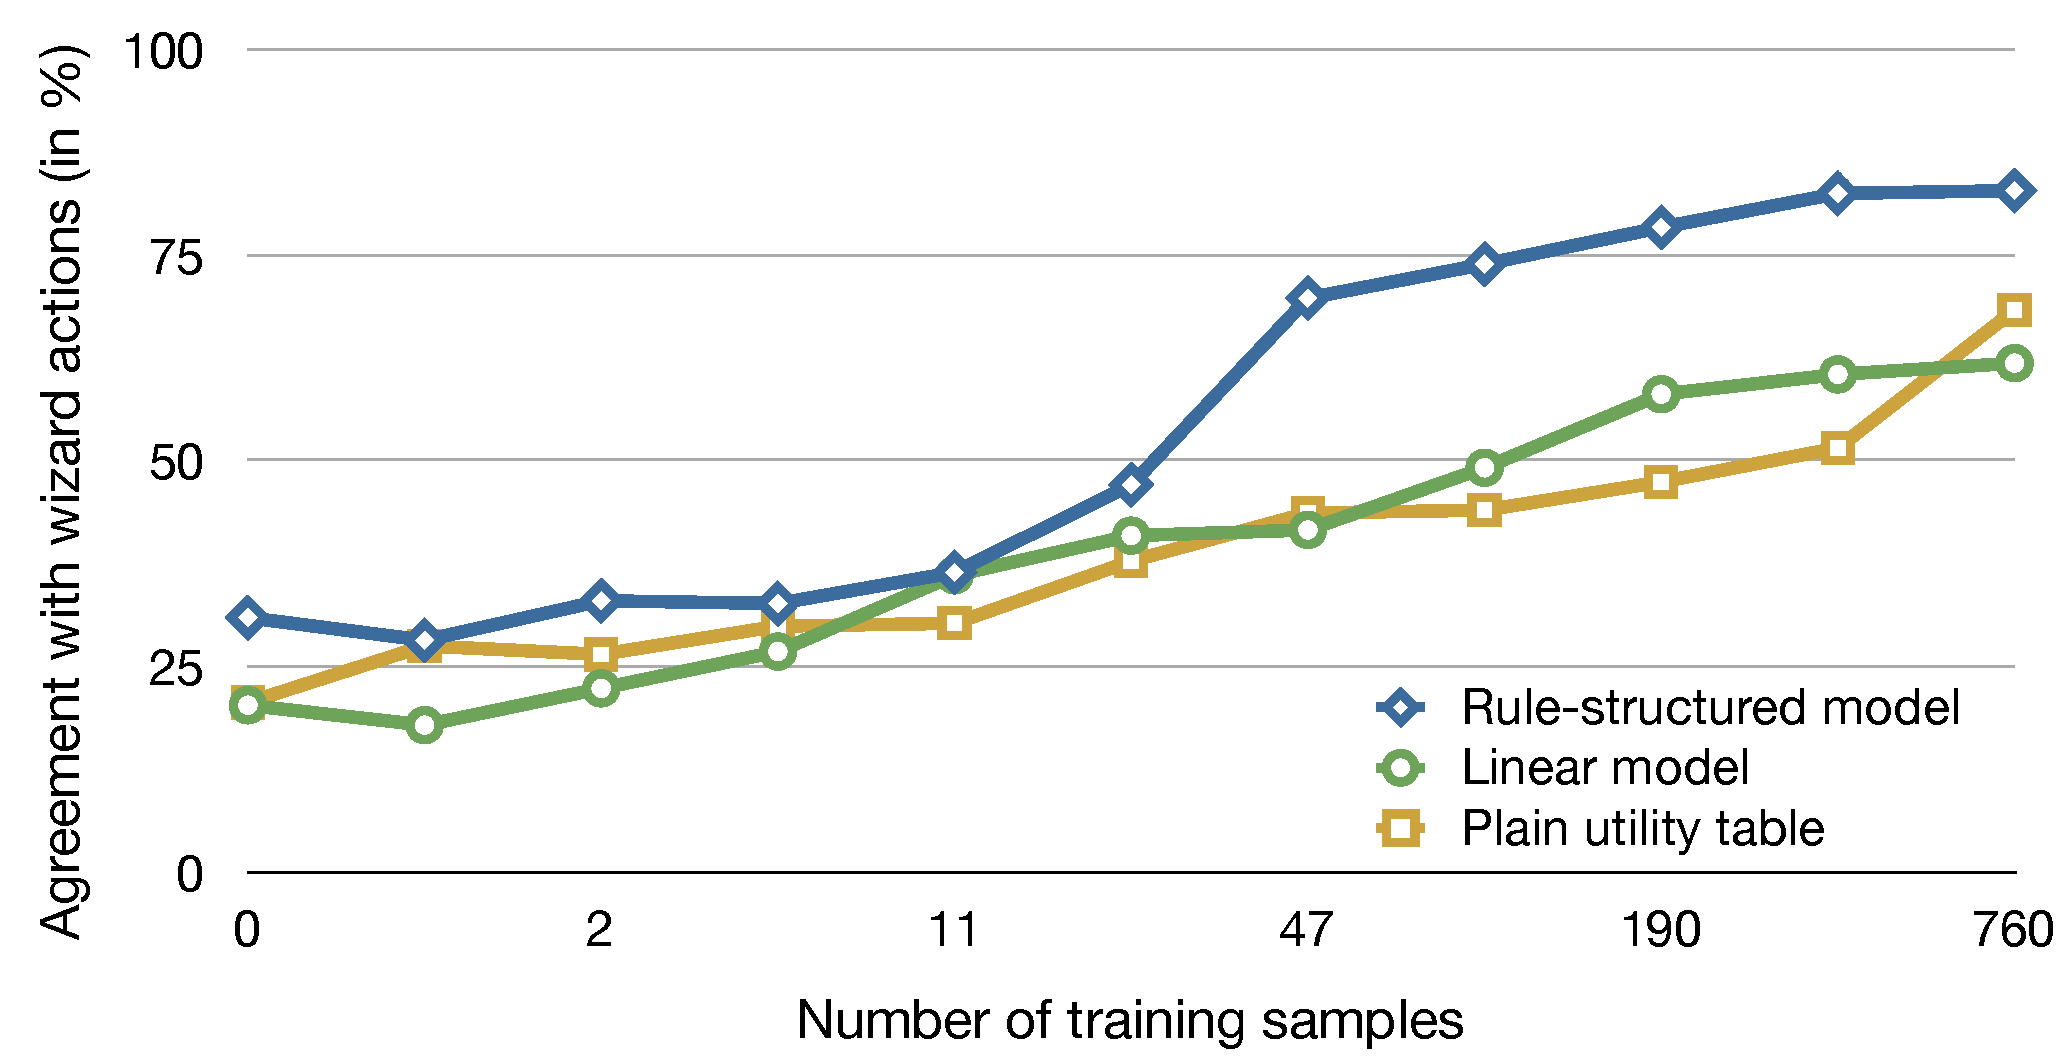
\includegraphics[scale=0.38]{imgs/results_log.pdf}
}\end{center}
\caption{Learning curves for the three utility models on the test set as a function of the number of processed data points.  The agreement results are given for the plain, linear and rule-structured utility models, using both linear (top) and logarithmic scales (bottom).}
\label{results}
\end{figure*}


Thanks to its considerably reduced number of parameters, the rule-structured model is able to converge to near-optimal values after observing only a small fraction of the training set.  The incorporation of domain knowledge via the rule structure has a clearly beneficial effect on the learning performance and on the generalisation capacity of the model\index{generalisation capacity}.  As the figure shows, the two baseline models do also improve their accuracies over time, but at a much slower rate.   The linear model is comparatively faster than the plain model, but levels off towards the end. The suboptimal learning performance of the linear model is most likely due to the non-linearity of some dialogue strategies.  The plain model continues its convergence and would probably reach an agreement level similar to the rule-structured model if given much larger amounts of training data. 

The learning results are in line with our expectations based on the respective sizes of the parameter space for the three utility models, and are not \textit{per se} highly surprising.  The main lesson to draw from this experiment is, however, not the exact difference in agreement or learning rates for each particular model, but the demonstration that probabilistic rules can be successfully applied to structure a small but non-trivial dialogue domain and derive its parameters from collected interaction data.  Through the use of abstraction mechanisms such as partitioning and quantification, the experiment show that the utility rules specified for the domain can cover large regions of the problem space without degrading the accuracy of the model.  The utility model can hence be optimised with only modest amounts of in-domain data. 


\section{Conclusion}
\label{sec:woz-conclusions}

The present chapter has described how parameters could be included in the specification of probabilistic rules and estimated via Bayesian learning techniques.  Rule parameters can represent either probability or utility values. The estimation process operates by calculating posterior probability distributions over possible parameter values given the observed data set. The process is initiated with prior distributions such as Dirichlet priors for probability values and Gaussian or uniform priors for utilities. 

The main focus of the chapter was on supervised learning of rule parameters based on Wizard-of-Oz training data. We described how Wizard-of-Oz data can be practically collected and processed to yield data points encoded as pairs $\langle$dialogue state $\mathcal{B}_i$, wizard action $a_i\rangle$. These data points are used to progressively narrow down the spread of the posterior distributions to the values that provide the best fit for the observed wizard actions. 

This learning approach has been implemented in a end-to-end spoken dialogue system for human--robot interaction and validated in a proof-of-concept experiment.  The goal of the experiment was to estimate the utility values of various actions on the basis of a Wizard-of-Oz data set.  Three utility models were compared: a plain utility table, a linear model, and a model structured with utility rules. The analysis of the empirical results shows that the rule-structured model outperforms the two baselines in regards to learning rate and generalisation performance with limited amounts of training data.

The outcome of the experiment corroborates one of the central claims of this thesis -- namely, that hybrid approaches to dialogue modelling (and in particular the formalism of probabilistic rules developed in this thesis) are well suited to model dialogue domains that must simultaneously confront high levels of uncertainty and limited availability of in-domain dialogue data. In such situations, which are commonplace in the field of spoken dialogue systems, neither purely symbolic nor purely data-driven approaches are alone sufficient to harness the complex and stochastic nature of the interactions.  Hybrid approaches to dialogue modelling provide ways to combine expert knowledge and statistically optimised parameters in a single, unified framework, thereby allowing the domain models to be tuned from even small amounts of training data. 

As shown in the experiments, Wizard-of-Oz interaction data can be a useful and interesting source of domain knowledge for the estimation of probabilistic models of dialogue. The data collection procedure can, however, be a tedious endeavour, as it requires:
\begin{enumerate}
\item The availability of an expert (the wizard) that can control the system and provide examples of appropriate behaviour for the domain.
\item The technical setup of a Wizard-of-Oz environment from which the wizard can perceive the user inputs, monitor contextual features, select possible actions to execute, and get all relevant information recorded and stored in a generic format. 
\end{enumerate}

A natural alternative to supervised learning from Wizard-of-Oz data is to let the dialogue system learn the best conversational behaviour via trial and error from its own interaction experience (that is, through reinforcement learning), without relying on the provision of external examples.\index{reinforcement learning}  The next chapter demonstrates how such a strategy can be practically implemented, based once again on the formalism of probabilistic rules to structure the domain models. 
